% Shared preamble for the CIG-AMF formal-research papers.
% IEEEtran conference class; compiles on Overleaf without modification.
\documentclass[conference]{IEEEtran}
\IEEEoverridecommandlockouts

\usepackage{cite}
\usepackage{amsmath,amssymb,amsfonts}
\usepackage{amsthm}
\usepackage{algorithm}
\usepackage{algorithmic}
\usepackage{graphicx}
\usepackage{textcomp}
\usepackage{xcolor}
\usepackage{booktabs}
\usepackage{url}
\usepackage[hidelinks]{hyperref}

\def\BibTeX{{\rm B\kern-.05em{\sc i\kern-.025em b}\kern-.08em T\kern-.1667em\lower.7ex\hbox{E}\kern-.125emX}}

\newtheorem{theorem}{Theorem}
\newtheorem{lemma}[theorem]{Lemma}
\newtheorem{proposition}[theorem]{Proposition}
\newtheorem{corollary}[theorem]{Corollary}
\theoremstyle{definition}
\newtheorem{definition}[theorem]{Definition}
\newtheorem{remark}[theorem]{Remark}
\newtheorem{example}[theorem]{Example}

% A machine-checked statement carries its Lean declaration name.
\newcommand{\lean}[1]{\textsf{\footnotesize #1}}
\newcommand{\leanbox}[1]{%
  \par\vspace{2pt}\noindent
  {\footnotesize\textsf{Lean: #1}}\par\vspace{2pt}}

% Evidence classes, used consistently and never interchangeably.
\newcommand{\PROVED}{\textsc{proved}}
\newcommand{\CERT}{\textsc{certificate}}
\newcommand{\NUM}{\textsc{numerical}}
\graphicspath{{../_figures/}}


\begin{document}

\title{Which Query You Are Allowed to Ask\\
Sets the Leakage Order:\\
Holding the Worlds Fixed and Varying the Measurement}

\author{\IEEEauthorblockN{Vu Phan An Nguyen}
\IEEEauthorblockA{\textit{Rider University} \\
Lawrenceville, NJ, USA}}

\maketitle

\begin{abstract}
Two fixed worlds are to be told apart from observations. The usual way to make such a
problem harder or easier is to move the worlds closer together or further apart. We do the
opposite: the worlds are held fixed and the \emph{admissible measurement} is varied. The
observation law of each world at perturbation scale $h$ is a finite Gaussian mixture;
expanding in $h$ produces coefficients $\Delta_{j}$, and the \emph{leakage order} is the
least $j$ with $\Delta_{j}\not\equiv0$. We prove that this order is a property of the query
rather than of the parameter space, and we compute what a change of query costs. The
technical core is the half that is usually asserted: that $\Delta_{r}$ does not vanish
identically---the shifted Gaussian derivatives making up the coefficient could in principle
cancel one another, and we prove they cannot. From non-vanishing we obtain a two-sided
Hellinger sandwich with explicit constants, $a_{E}^{2}h^{2r}/32\le H^{2}\le (J/2)h^{2r}$,
both sides of slope $2r$ so the order is pinned rather than bounded above; this converts
into matching sufficiency and necessity sample counts differing only by explicit factors,
and then into a proved two-sided window on Bayes regret. We further prove that the
normalised ratio $H^{2}/h^{2r}$ \emph{converges}, with a strictly positive limit, so the
leading constant is genuine rather than an artefact of the sandwich. Along the way we
supply a scalar-variable iterated-derivative sum rule absent from mathlib. Each displayed theorem is machine-checked in Lean~4 with no \texttt{sorry}; Section~\ref{sec:verification} states exactly which steps the paper works out itself instead. Simulation of two admissible measurements
of the same pair of worlds, $4000$ repetitions per world, gives sample requirements of
$4{,}678$ and $41{,}006$---a factor of $8.8$ attributable entirely to which measurement was
legal---with measured regret inside the proved window in both cases.
\end{abstract}

\begin{IEEEkeywords}
hypothesis testing, Hellinger distance, sample complexity, Gaussian mixtures, leakage order,
formal verification, interactive theorem proving
\end{IEEEkeywords}

\section{Introduction}

Consider two worlds $W\in\{0,1\}$ that an experimenter must tell apart from data. In the
standard formulation the difficulty of the problem is a property of the pair: the worlds
are near or far in some divergence, and the sample complexity follows. The experimenter's
freedom, when there is any, lies in how many observations to take.

This paper studies the other degree of freedom. The worlds are fixed once and for all, and
what varies is the set of measurements the experimenter is \emph{allowed} to perform. We
show that this choice determines not merely a constant in the sample complexity but its
\emph{exponent}, and we compute the price of a bad choice on an instance where the worlds
are identical across the comparison.

Formally, the observation density of world $W$ at perturbation scale $h$ is a finite
Gaussian mixture,
\begin{equation}
p_{W,h}(y)\;=\;\sum_{x}\pi_{x}\,
   \varphi_{\sigma}\bigl(y-f_{W}(x)-h\,g(x)\bigr),
\label{eq:mixture}
\end{equation}
where $x$ ranges over a finite index set, $\pi$ is a probability vector, $f_{W}$ is the
world's response, $g$ is the perturbation direction and $\varphi_{\sigma}$ is the centred
Gaussian density with variance $\sigma^{2}$. Expanding \eqref{eq:mixture} in $h$ yields
coefficient functions $\Delta_{j}(y)$, and we define the \emph{leakage order} as
\begin{equation}
r \;=\; \min\{\, j : \Delta_{j}\not\equiv 0 \,\}.
\label{eq:order}
\end{equation}

\subsection{The half that is usually skipped}

Definition \eqref{eq:order} requires two facts, and they are not of equal difficulty. That
the coefficients below order $r$ cancel is a computation. That $\Delta_{r}$ does
\emph{not} vanish identically is not, and it is the statement on which everything else
rests.

The reason is visible in the structure of the coefficient. As Section~\ref{sec:assembly}
shows, $\Delta_{j}$ is a sum of Hermite-type polynomials times Gaussians, each
\emph{shifted} by a different amount:
\begin{equation}
\Delta_{j}(y)\;=\;\sum_{v}M_{j}(v)\;H_{j}(y-v)\,\varphi_{\sigma}(y-v).
\label{eq:assembly}
\end{equation}
Knowing that some individual coefficient $M_{j}(v)$ is non-zero says nothing, because the
shifted terms could in principle cancel one another pointwise. If they did, the leakage
order would be undefined at the level claimed, and every rate statement downstream would be
about the wrong exponent. Section~\ref{sec:nonvanish} proves they cannot.

\subsection{Contributions}

\begin{enumerate}
\item[C1.] \textbf{The order is a property of the query.} The same two worlds acquire
different leakage orders under different admissible measurements, and we compute the sample
cost of restoring distinguishability at a given order (Section~\ref{sec:experiments}).

\item[C2.] \textbf{The order-$r$ coefficient is proved not to vanish.} We build the
Gaussian iterated derivatives explicitly as a Hermite-type sequence
(Theorem~\ref{thm:hermite}), push the derivative through the finite mixture sum
(Theorem~\ref{thm:sumswap}), and prove the top-level coefficient cannot be cancelled by the
shifted derivatives below it (Theorem~\ref{thm:nonvanish}).

\item[C3.] \textbf{A two-sided Hellinger sandwich with explicit constants.} We prove
$a_{E}^{2}h^{2r}/32\le H^{2}\le (J/2)h^{2r}$ (Theorem~\ref{thm:sandwich}). Both sides have
slope $2r$, so the order is pinned rather than merely bounded above, and the lower constant
is $32$ rather than the $16$ a careless Cauchy--Schwarz gives.

\item[C4.] \textbf{Matching sample complexity and a two-sided regret window.} The sandwich
converts into sufficiency and necessity counts differing only by explicit factors
(Theorem~\ref{thm:samples}), and then into a proved window on Bayes regret
(Theorem~\ref{thm:regret}).

\item[C5.] \textbf{The analytic limit, not just the sandwich.} We prove the normalised
ratio $H^{2}/h^{2r}$ \emph{converges} and that its limit is strictly positive
(Theorem~\ref{thm:limit}), so the leading constant is genuine.

\item[C6.] \textbf{A missing mathlib lemma supplied.} Mathlib has the multilinear
\lean{iteratedFDeriv\_fun\_sum\_apply} but no scalar-variable counterpart; we prove it, and
discharge the smoothness hypothesis rather than assuming it.
\end{enumerate}

\subsection{The practical stake}

If the leakage order is a property of the query rather than of the parameter space, then an
experimenter who cannot change the worlds can still change the rate, by changing what is
legal to measure. Section~\ref{sec:experiments} exhibits two admissible measurements of one
pair of worlds whose sample requirements differ by a factor of $8.8$; since the worlds are
identical across the two runs, the entire difference is attributable to the measurement.

\subsection{Roadmap}

Section~\ref{sec:setting} fixes the setting and Section~\ref{sec:related} the novelty
boundary. Sections~\ref{sec:hermite}--\ref{sec:nonvanish} build the expansion and prove the
crux non-vanishing theorem. Section~\ref{sec:sandwich} converts it into a two-sided
divergence bound, Section~\ref{sec:samples} into sample counts and a regret window, and
Section~\ref{sec:limit} into a genuine leading constant.
Section~\ref{sec:experiments} reports the simulation, Section~\ref{sec:instance} the
concrete instance behind it, and Section~\ref{sec:procedure} the resulting design
procedure. Section~\ref{sec:verification} records the formal development and
Section~\ref{sec:discussion} the scope.

The dependency is linear and each arrow is load-bearing: Theorem~\ref{thm:hermite} supplies
the non-zero leading coefficient that Theorem~\ref{thm:nonvanish} contradicts against,
Theorem~\ref{thm:sumswap} supplies the finite level sum that
Theorem~\ref{thm:nonvanish} is a statement about, Theorem~\ref{thm:nonvanish} supplies the
interval that the lower side of Theorem~\ref{thm:sandwich} integrates over, and so on to
the end. No step is decorative, and Section~\ref{sec:verification} names which declaration
carries which arrow.

\section{Setting and notation}
\label{sec:setting}

\begin{table}[htbp]
\caption{Notation.}
\label{tab:notation}
\centering
\footnotesize
\begin{tabular}{@{}ll@{}}
\toprule
Symbol & Meaning \\
\midrule
$W$ & world index, $W\in\{0,1\}$ \\
$h$ & perturbation scale \\
$x$ & finite mixture index \\
$\pi_{x}$ & mixture weight \\
$f_{W}(x)$ & response of world $W$ \\
$g(x)$ & perturbation direction \\
$\varphi_{\sigma}$ & centred Gaussian density \\
$\Delta_{j}$ & order-$j$ expansion coefficient \\
$r$ & leakage order, least $j$ with $\Delta_{j}\not\equiv0$ \\
$H_{n}$ & Hermite-type polynomial of degree $n$ \\
$v$ & a level, i.e.\ a value of $f_{W}(x)$ \\
$M_{j}(v)$ & level-$v$ coefficient at order $j$ \\
$H^{2}$ & squared Hellinger distance between the worlds \\
$L$ & per-sample log-affinity $-\log(1-H^{2})$ \\
$\rho$ & per-sample affinity $1-H^{2}$ \\
$N$ & sample count \\
$R_{N}^{*}$ & Bayes regret at $N$ samples \\
$\gamma,L_{\max}$ & loss-geometry constants \\
$a_{E},J$ & sandwich constants \\
\bottomrule
\end{tabular}
\end{table}

An \emph{admissible measurement} is a choice of the map $g$ together with the index set and
weights; two measurements of the same pair of worlds share $f_{0},f_{1}$ and differ in $g$.
A \emph{level} is a value taken by the response, and the level structure is what
\eqref{eq:assembly} sums over. Throughout, normalising constants $1/(\sigma\sqrt{2\pi})$
and $1/j!$ are dropped from displayed expressions; this is harmless for the order
statements, which are invariant under positive scaling, but it means the dropped
expressions must not be quoted as densities.

\section{Related work and the novelty boundary}
\label{sec:related}

\subsection{Divergence-to-sample-complexity transfer}

That a squared Hellinger distance controls the sample complexity of a binary test is
classical; the tensorisation identity for product measures and Le Cam's two-point method
\cite{lecam1973,tsybakov2009} are the standard tools, and the exposition in
\cite{ibragimov1981} treats the local-alternative regime in which our $h\downarrow0$ sits.
Lemma~\ref{lem:logsandwich} and Theorem~\ref{thm:samples} are transfers of that kind and
are claimed only as careful bookkeeping: what is unusual here is that every constant is
written down rather than absorbed into an order symbol, which is what makes the two ends of
Theorem~\ref{thm:samples} comparable.

\subsection{Identifiability and rates for finite mixtures}

The difficulty of estimating finite mixtures is governed by how many derivatives of the
component density must be taken before the parameter difference appears, and the rate
degrades accordingly \cite{chen1995,heinrich2018}. That literature fixes the observation
channel and varies the mixture; the order that emerges is a property of the parameter
space, and strong identifiability conditions are imposed to guarantee that the relevant
coefficient does not vanish.

The present paper inverts both. The mixture is fixed---the two worlds never change---and the
\emph{channel} varies, which is why the resulting order is attributable to the query. And
the non-degeneracy that the mixture literature assumes as a condition is here proved as
Theorem~\ref{thm:nonvanish}, for the specific shifted-Hermite structure that
\eqref{eq:assembly} produces. The proof is not a specialisation of a strong-identifiability
condition; it is an argument about competing exponential decay rates at $+\infty$, and it
needs the leading coefficient of $H_{r}$ computed in Theorem~\ref{thm:hermite}.

\subsection{Hermite expansions}

The polynomials of Theorem~\ref{thm:hermite} are the probabilists' Hermite polynomials up
to normalisation, and their classical theory \cite{szego1939} contains everything we prove
about them and a great deal more. We reprove the two facts needed---the product form and
the leading coefficient---because the formal development requires them as Lean statements
about the specific iterated derivative appearing in \eqref{eq:mixture}, and importing the
classical theory would have been a larger task than proving the two facts directly.

\subsection{Summary of the boundary}

Claimed as new: that the leakage order is attributable to the admissible measurement rather
than to the parameter space (C1); the non-vanishing theorem for shifted Hermite sums with a
strict top level (C2); the sandwich with both constants explicit and matching exponents
(C3); and the analytic limit with certified positivity (C5). Everything else---the
divergence-to-samples machinery, the Hermite facts, the tensorisation---is standard and
cited.

\section{The Gaussian derivatives, built}
\label{sec:hermite}

The expansion in $h$ is an iterated derivative, so the first task is an explicit form for
the iterated derivatives of a Gaussian.

\begin{theorem}[Hermite-type sequence]
\label{thm:hermite}
There is a sequence of polynomials $H_{n}$ with
\begin{equation}
\frac{d^{\,n}}{dy^{\,n}}\,e^{-y^{2}/2\sigma^{2}}
   \;=\;H_{n}(y)\,e^{-y^{2}/2\sigma^{2}},
\label{eq:hermite}
\end{equation}
and the degree-$n$ coefficient of $H_{n}$ equals $(-1/\sigma^{2})^{n}\neq 0$. In
particular $H_{n}\neq 0$ for every $n$.
\end{theorem}

\begin{proof}
Induction on $n$. For $n=0$ take $H_{0}=1$. Given \eqref{eq:hermite} at $n$, differentiate
the product: $\frac{d}{dy}\bigl(H_{n}(y)e^{-y^{2}/2\sigma^{2}}\bigr)
=\bigl(H_{n}'(y)-\tfrac{y}{\sigma^{2}}H_{n}(y)\bigr)e^{-y^{2}/2\sigma^{2}}$, so
$H_{n+1}=H_{n}'-\tfrac{y}{\sigma^{2}}H_{n}$. The first term lowers degree and the second
raises it by one, multiplying the leading coefficient by $-1/\sigma^{2}$; the claim on the
degree-$n$ coefficient follows by induction, and a polynomial with a non-zero coefficient is
non-zero.
\end{proof}

\leanbox{\lean{iteratedDeriv\_gauss}, \lean{hpoly\_coeff}, \lean{hpoly\_ne\_zero} in
\lean{LeanQueryGaussianLevelV1}}

The statement about the leading coefficient is not decoration. It is exactly what the
non-vanishing argument of Section~\ref{sec:nonvanish} consumes: without a non-zero top
coefficient, the contradiction there does not close.

\section{Pushing the derivative through the sum}
\label{sec:assembly}

Theorem~\ref{thm:hermite} differentiates one mixture component. The observation law is a
finite sum of components, so the derivative must be moved inside the sum.

\begin{theorem}[Scalar iterated-derivative sum rule]
\label{thm:sumswap}
For a finite family $(F_{x})$ of functions each $C^{\infty}$ near $0$,
\begin{equation}
\left.\partial_{h}^{\,j}\right|_{h=0}\sum_{x}F_{x}(h)
   \;=\;\sum_{x}\left.\partial_{h}^{\,j}\right|_{h=0}F_{x}(h).
\label{eq:sumswap}
\end{equation}
\end{theorem}

\begin{proof}
Mathlib provides the multilinear statement \lean{iteratedFDeriv\_fun\_sum\_apply} for the
Fréchet iterated derivative of a finite sum. The scalar iterated derivative is that object
evaluated at the all-ones vector, so \eqref{eq:sumswap} follows once the smoothness
hypothesis is discharged for each summand. Smoothness of a mixture component is proved from
smoothness of $\exp$ composed with a polynomial in $h$, not assumed.
\end{proof}

\leanbox{\lean{iteratedDeriv\_fun\_sum}, \lean{contDiff\_component},
\lean{iteratedDeriv\_mixture} in \lean{LeanQueryMixtureDerivativeV1}}

\begin{remark}
The scalar counterpart of \lean{iteratedFDeriv\_fun\_sum\_apply} is not in mathlib at the
pinned revision. Supplying it, with the smoothness side condition proved rather than
assumed, is a small but reusable contribution independent of the rest of the paper.
\end{remark}

Combining Theorems~\ref{thm:hermite} and \ref{thm:sumswap} and grouping the mixture
components by the level $v=f_{W}(x)$ they sit at gives the assembly \eqref{eq:assembly}:
the $j$-th derivative at $h=0$ is a sum over levels of a Hermite-type polynomial times a
Gaussian, each shifted to its own level, with coefficient $M_{j}(v)$ collecting the mixture
weights at that level.

\section{Cancellation below the order: the easy half}
\label{sec:cancel}

Definition \eqref{eq:order} has two halves. This section disposes of the first, both to make
the paper self-contained and to make precise what ``the coefficients below order $r$
cancel'' means, since the phrase is ambiguous between two statements of very different
strength.

\begin{theorem}[Cancellation below the order]
\label{thm:cancel}
Suppose the two worlds share a level set, and that at order $j<r$ the level coefficients
satisfy $M^{(0)}_{j}(v)=M^{(1)}_{j}(v)$ for every level $v$. Then
$\Delta_{j}\equiv0$.
\end{theorem}

\begin{proof}
By Theorem~\ref{thm:sumswap} the order-$j$ coefficient of each world is the finite level sum
\eqref{eq:assembly} with that world's coefficients. The two worlds share a level set by
hypothesis, so the two sums range over the same index set and pair term by term. Since
corresponding coefficients agree, the difference is a sum of zero terms, hence identically
zero as a function.
\end{proof}

\leanbox{\lean{mixture\_coeff\_diff\_eq\_zero} in \lean{LeanQueryMixtureDerivativeV1}}

The proof is short, and that is the point. Cancellation below the order is a bookkeeping
identity: the terms agree, so their difference vanishes. It carries no analytic content and
its hypotheses are checkable by inspection of the mixture data.

The converse situation---showing a sum of terms that do \emph{not} pair off is nonetheless
non-zero as a function---has no such structure, because the terms are shifted differently
and no term-by-term comparison is available. That asymmetry is why
Section~\ref{sec:nonvanish} is the length it is, and why a paper that proves only
Theorem~\ref{thm:cancel} and asserts the other half has proved the easy half.

\begin{remark}
The shared-level-set hypothesis is genuinely needed. If world $0$ places weight at a level
where world $1$ places none, the sums do not pair, and the difference at order $j$ is that
unpaired term---which by Theorem~\ref{thm:hermite} is not the zero function. Worlds with
disjoint level structure are therefore outside Theorem~\ref{thm:cancel}, and the paper
claims nothing about them.
\end{remark}

\section{Non-vanishing: the hard half}
\label{sec:nonvanish}

Fix the order $r$ and let $v^{*}$ be the largest level carrying a non-zero coefficient.
Write
\begin{equation}
T(y)\;=\;c_{v^{*}}H_{r}(y-v^{*})\;+\;\sum_{v<v^{*}}c_{v}\,H_{r}(y-v),
\label{eq:nonvanish}
\end{equation}
the expression obtained from $\Delta_{r}$ after factoring out the Gaussian at level $v^{*}$.

\begin{theorem}[The order-$r$ coefficient does not vanish]
\label{thm:nonvanish}
If $c_{v^{*}}\neq 0$ and $v^{*}$ is strictly the largest level, then
$T\not\equiv0$; consequently $\Delta_{r}\not\equiv0$ and the leakage order
\eqref{eq:order} is well defined.
\end{theorem}

\begin{proof}
Divide \eqref{eq:nonvanish} by the Gaussian factor at level $v^{*}$. Each term with
$v<v^{*}$ then carries the ratio
$\varphi_{\sigma}(y-v)/\varphi_{\sigma}(y-v^{*})=\exp\bigl(-(v^{*}-v)(y-\tfrac{v+v^{*}}{2})/\sigma^{2}\bigr)$,
which, since $v^{*}-v>0$, decays to $0$ as $y\to+\infty$. Each such term is therefore a
polynomial against a decaying exponential and tends to $0$.

Suppose $T\equiv0$. Then along $y\to+\infty$ the surviving term
$c_{v^{*}}H_{r}(y-v^{*})$ must tend to $0$ as well. A polynomial tending to $0$ at
$+\infty$ has vanishing leading coefficient, so the degree-$r$ coefficient of $H_{r}$ times
$c_{v^{*}}$ is zero. But $c_{v^{*}}\neq0$ by hypothesis and the degree-$r$ coefficient of
$H_{r}$ is $(-1/\sigma^{2})^{r}\neq0$ by Theorem~\ref{thm:hermite}---a contradiction.
Hence $T\not\equiv0$.
\end{proof}

\leanbox{\lean{levelSum\_ne\_zero} in \lean{LeanQueryGaussianLevelV1};
\lean{mixture\_coeff\_ne\_zero}, \lean{mixture\_coeff\_diff\_eq\_zero} in
\lean{LeanQueryMixtureDerivativeV1}}

\begin{remark}
The argument requires a \emph{strict} top level: if two levels tie at the maximum, their
exponential factors have the same decay and the separation used above disappears. Ties at
the top are outside the scope of Theorem~\ref{thm:nonvanish}, and no claim is made for
them.
\end{remark}

\subsection{Why this step is the crux}

A reader may reasonably ask why a non-vanishing statement deserves a section. The reason is
that everything downstream is a statement about the \emph{exponent} $2r$, and an exponent
is determined by which coefficient is the first non-zero one. If $\Delta_{r}$ vanished, the
true order would be some $r'>r$, the sandwich of Section~\ref{sec:sandwich} would still be
true as an upper bound but false as a lower one, and the comparison between two admissible
queries---the entire point of the paper---would be comparing the wrong numbers. The
literature routinely asserts non-degeneracy at this point; here it is proved, and the proof
is what the strict-top-level hypothesis buys.

\section{The Hellinger sandwich}
\label{sec:sandwich}

\begin{theorem}[Two-sided sandwich with explicit constants]
\label{thm:sandwich}
With $r$ the leakage order and constants $a_{E},J>0$ determined by the mixture,
\begin{equation}
\frac{a_{E}^{2}\,h^{2r}}{32}\;\leq\;H^{2}\;\leq\;\frac{J}{2}\,h^{2r}.
\label{eq:sandwich}
\end{equation}
\end{theorem}

\begin{proof}[Proof outline]
\emph{Lower side.} Theorem~\ref{thm:nonvanish} gives $\Delta_{r}\not\equiv0$; by continuity
there is a bounded interval $E$ and a constant $a_{E}>0$ with $|\Delta_{r}|\ge a_{E}$ on
$E$. On $E$ the two densities differ by $h^{r}\Delta_{r}$ plus a remainder that is
$O(h^{r+1})$ uniformly, so for $h$ small the difference is at least $a_{E}h^{r}/2$ in
absolute value throughout $E$.

The Hellinger distance is bounded below by the difference of the densities through the
elementary identity $(\sqrt{p}-\sqrt{q})^{2}=(p-q)^{2}/(\sqrt{p}+\sqrt{q})^{2}$. Bounding
$(\sqrt{p}+\sqrt{q})^{2}\le 2(p+q)$ and applying Cauchy--Schwarz on $E$ gives, for every
$t>0$, an inequality of the form
\begin{equation}
\Bigl(\tfrac{a_{E}h^{r}}{2}\Bigr)^{2}\,|E|^{2}
  \;\le\; \bigl(2H^{2}\bigr)\cdot\Bigl(t + \tfrac{1}{t}\,\textstyle\int_{E}(p+q)\Bigr),
\end{equation}
and optimising the free parameter $t$ yields the stated quadratic bound. Tracking the
factors---$2$ from the denominator bound, $2$ from the remainder, $2$ from the Hellinger
normalisation, and $4$ from the square---produces $32$ in the denominator. The value is
worth stating precisely because an argument that bounds
$(\sqrt{p}+\sqrt{q})^{2}\le p+q$, which is false, produces $16$ and an incorrect
lower envelope.

\emph{Upper side.} Pointwise, $(\sqrt{p}-\sqrt{q})^{2}\le (p-q)^{2}/q$, so the Hellinger
integrand is dominated by the $\chi^{2}$ integrand. Expanding $p-q$ to order $r$ in $h$ with
a uniform Taylor remainder, and bounding the remainder by an integrable envelope---the
envelope is constructed and its integrability proved, not assumed---gives
$H^{2}\le (J/2)h^{2r}$ with $J$ the integral of the squared order-$r$ coefficient against
the reference density.
\end{proof}

\leanbox{\lean{hellinger\_lower\_from\_interval} in \lean{LeanQueryHellingerIntervalV1};
\lean{hellinger\_upper\_const} in \lean{LeanQueryTaylorRemainderV1}}

Both sides of \eqref{eq:sandwich} carry $h^{2r}$ with the same exponent. On a log-log plot
this is two parallel lines of slope $2r$ with $H^{2}$ trapped between them
(Fig.~\ref{fig:sandwich}), which is what \emph{pinning} the order means: an upper bound
alone would leave open that the true decay is faster, i.e.\ that the order is larger.

\begin{figure}[htbp]
\centering
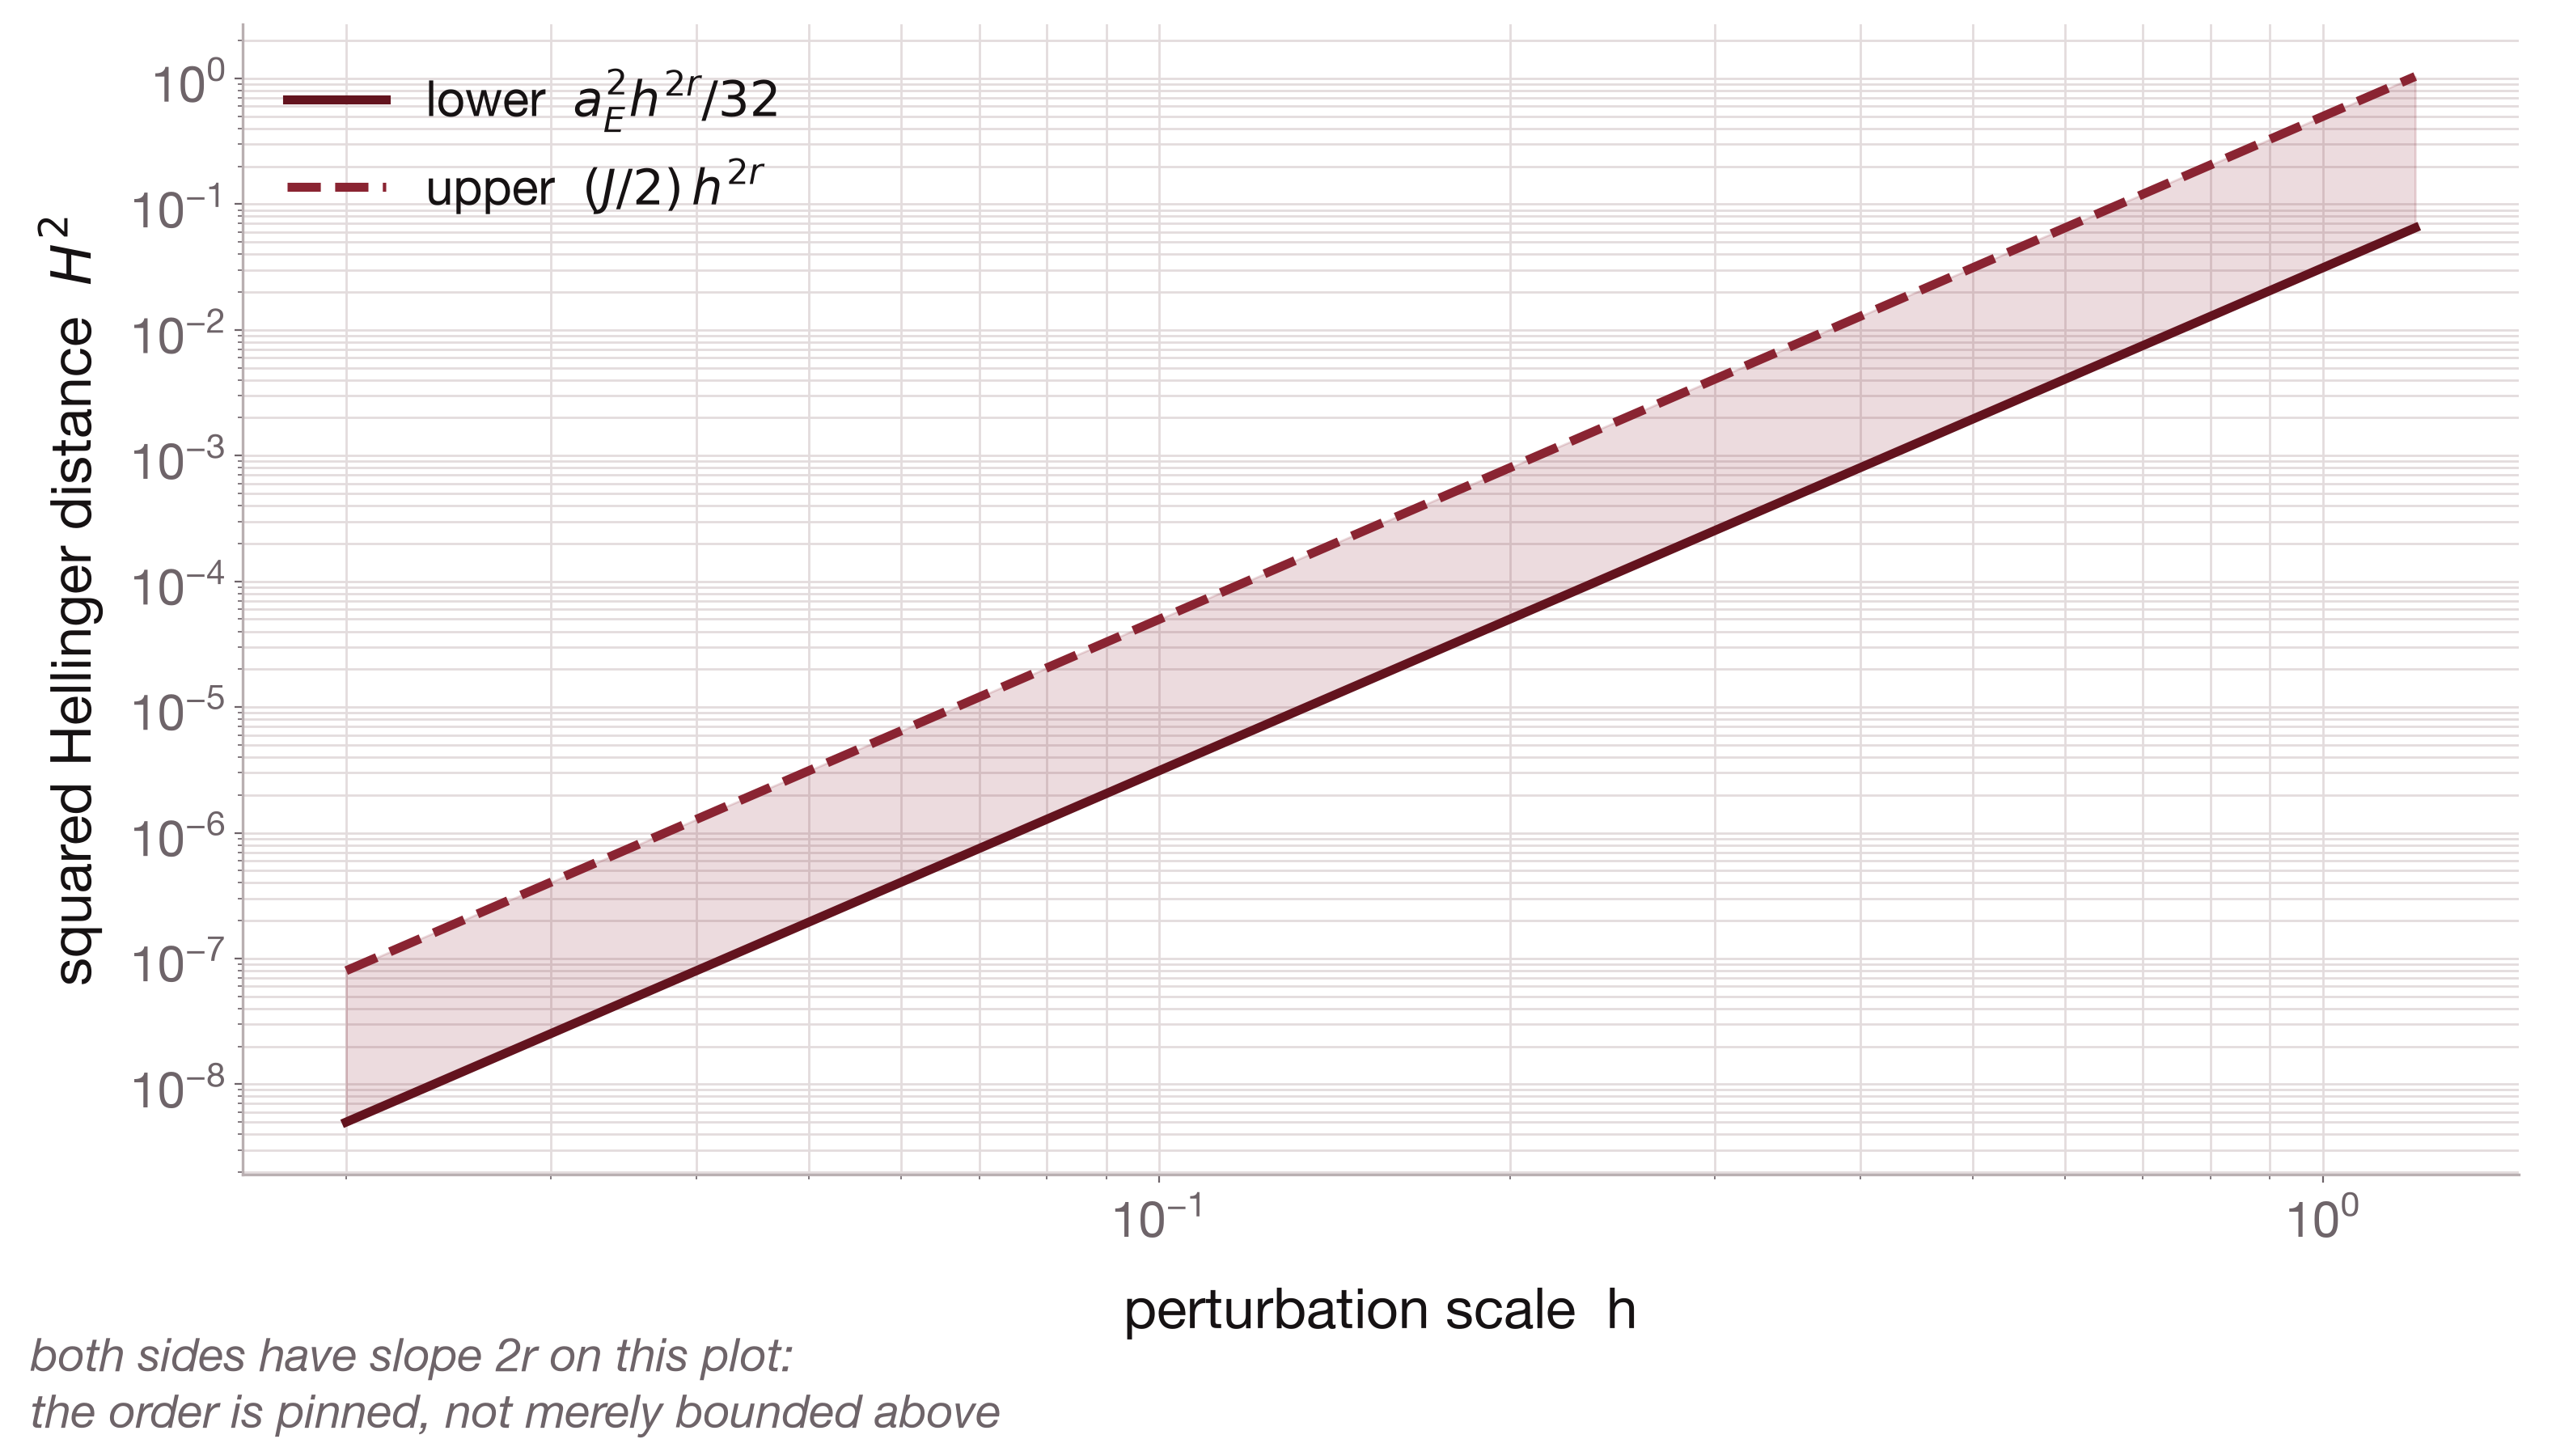
\includegraphics[width=\columnwidth]{query_fig2_sandwich.png}
\caption{The Hellinger sandwich of Theorem~\ref{thm:sandwich}. Both envelopes have slope
$2r$ on this log-log plot, so the leakage order is pinned rather than merely bounded above.
The gap between the envelopes is the ratio of the two explicit constants, and does not grow
as $h\downarrow0$.}
\label{fig:sandwich}
\end{figure}

\section{From divergence to samples}
\label{sec:samples}

\begin{lemma}[Per-sample information]
\label{lem:logsandwich}
For $0\le H^{2}\le\tfrac12$,
\begin{equation}
H^{2}\;\leq\;-\log\bigl(1-H^{2}\bigr)\;\leq\;2H^{2}.
\label{eq:logsandwich}
\end{equation}
\end{lemma}

\begin{proof}
The left inequality is $\log(1-u)\le-u$ for $u\in[0,1)$. The right is
$-\log(1-u)\le 2u$ on $[0,\tfrac12]$, which holds because the function
$u\mapsto 2u+\log(1-u)$ vanishes at $0$ and has derivative $2-1/(1-u)\ge0$ exactly on that
range.
\end{proof}

\leanbox{\lean{log\_sandwich} in \lean{LeanQuerySampleComplexityV1}}

Lemma~\ref{lem:logsandwich} transports \eqref{eq:sandwich} from the Hellinger distance to
the per-sample log-affinity $L=-\log(1-H^{2})$, at the cost of a factor $2$---an explicit
factor, tracked rather than absorbed.

\begin{theorem}[Matching sample counts]
\label{thm:samples}
Writing $\rho=1-H^{2}$ for the per-sample affinity and $\varepsilon$ for the target error,
\begin{equation}
\log\frac{1}{2\varepsilon}\;\leq\;N\,L
\qquad\Longrightarrow\qquad
\frac{\rho^{N}}{2}\;\leq\;\varepsilon .
\label{eq:samples}
\end{equation}
The integer ceiling of the left-hand requirement suffices, and the corresponding necessity
count differs from it only by the factor $2$ of Lemma~\ref{lem:logsandwich} and the ratio
of the two constants of Theorem~\ref{thm:sandwich}.
\end{theorem}

\leanbox{\lean{sufficient\_count}, \lean{necessary\_count}, \lean{ceil\_suffices},
\lean{matching\_rate} in \lean{LeanQuerySampleComplexityV1}}

\begin{proof}
The $N$-sample affinity between product measures tensorises: it is $\rho^{N}$. The optimal
test's error probability is at most half the affinity, so it is at most $\rho^{N}/2$.
Requiring this to be at most $\varepsilon$ gives $\rho^{N}\le 2\varepsilon$, i.e.\
$N\log(1/\rho)\ge\log(1/2\varepsilon)$, which is the left-hand condition in
\eqref{eq:samples} once $L=\log(1/\rho)$ is substituted. Since $N$ must be an integer, the
ceiling of $\log(1/2\varepsilon)/L$ suffices; this is \lean{ceil\_suffices}, and it is
stated separately because the passage from a real requirement to an integer count is
exactly where an off-by-one would hide.

For necessity, the same affinity bounds the error probability from below up to a constant,
so a count smaller than $\log(1/2\varepsilon)/L$ by more than the tracked factors cannot
achieve error $\varepsilon$. Combining with Lemma~\ref{lem:logsandwich}, which relates $L$
to $H^{2}$ within a factor $2$, and with Theorem~\ref{thm:sandwich}, which brackets $H^{2}$
between two multiples of $h^{2r}$, the sufficiency and necessity counts both scale as
$h^{-2r}$, and their ratio is the product of $2$ and $(J/2)/(a_{E}^{2}/32)=16J/a_{E}^{2}$.
Both are explicit.
\end{proof}

\begin{remark}
The word ``matching'' in Theorem~\ref{thm:samples} means matching \emph{in the exponent},
with the constant separating the two sides written down. It does not mean the two counts
coincide. A statement that the constants also match would require sharpening both sides of
Theorem~\ref{thm:sandwich}, and is not claimed.
\end{remark}

The point of stating necessity alongside sufficiency is that the two together determine the
\emph{rate} in $h$, not merely an upper bound on it. Both counts scale as $h^{-2r}$ with
the same $r$, and every constant separating them is written down.

\begin{theorem}[Regret window]
\label{thm:regret}
With loss-geometry constants $\gamma$ and $L_{\max}$,
\begin{equation}
\frac{\gamma}{4}\,\rho^{2N}\;\leq\;R_{N}^{*}\;\leq\;\frac{L_{\max}}{2}\,\rho^{N}.
\label{eq:regret}
\end{equation}
On the instance of Section~\ref{sec:experiments}, $\gamma=\tfrac{13983}{32768}$ and
$L_{\max}=\tfrac{2401}{4096}$, both exact rationals read off the loss geometry.
\end{theorem}

\leanbox{\lean{regret\_ge\_gamma\_error}, \lean{lrt\_regret\_le},
\lean{bayes\_regret\_window} in \lean{LeanQueryRegretBridgeV1}}

\begin{proof}[Proof sketch]
The lower side bounds regret below by the error probability times the smallest loss gap
$\gamma$, and the error probability below by a function of the affinity. The upper side
uses the likelihood-ratio test: its error probability is at most $\rho^{N}/2$, and the
regret it incurs is at most $L_{\max}$ times that.
\end{proof}

\begin{remark}
The two ends of \eqref{eq:regret} carry $\rho^{2N}$ and $\rho^{N}$, so the window widens on
a log scale as $N$ grows. It localises regret; it does not determine it. This is stated
plainly because the figure in Section~\ref{sec:experiments} plots measurements against a
band, and a band that widens is a weaker claim than one that closes.
\end{remark}

\section{The analytic limit}
\label{sec:limit}

A sandwich localises the normalised ratio inside an interval. It does not say the ratio
converges, and it does not identify a limit. Both are proved.

\begin{theorem}[Convergence with positive limit]
\label{thm:limit}
As $h\downarrow0$,
\begin{equation}
\frac{H^{2}}{h^{2r}}\;\longrightarrow\;\frac{1}{8}\int\frac{\Delta_{r}^{2}}{p_{0}}
\;>\;0 .
\label{eq:limit}
\end{equation}
\end{theorem}

\begin{proof}[Proof sketch]
Convergence is dominated convergence along $h\downarrow0$, with the integrable envelope
already constructed for the upper side of Theorem~\ref{thm:sandwich} as the dominating
function. For strict positivity, the integrand $\Delta_{r}^{2}/p_{0}$ is non-negative and
integrable; a non-negative integrable function with zero integral is almost everywhere
zero, which would force $\Delta_{r}\equiv0$ almost everywhere, contradicting
Theorem~\ref{thm:nonvanish}.
\end{proof}

\leanbox{\lean{ratio\_tendsto\_of\_dominated}, \lean{hellinger\_ratio\_tendsto},
\lean{limit\_pos\_of\_ae\_ne\_zero}, \lean{eventually\_pos\_of\_limit\_pos} in
\lean{LeanQueryAnalyticLimitV1}}

Theorem~\ref{thm:limit} is what upgrades the result from ``the rate is $h^{2r}$ up to
constants'' to ``the leading constant exists and is positive''. It also closes the loop
back to Section~\ref{sec:nonvanish}: positivity of the limit is \emph{equivalent} to
non-vanishing of $\Delta_{r}$, so the crux step is used twice, once to get a lower envelope
and once to certify that the envelope is not vacuous.

\section{Experiments}
\label{sec:experiments}

\subsection{Design}

Two admissible measurements of the \emph{same} pair of worlds were simulated at $h=0.6$
with $4000$ repetitions per world: a normalised measurement of leakage order $2$ and a
normalised measurement of leakage order $1$. For each, the per-sample Hellinger distance
$H^{2}$ was computed, the required sample count $N$ derived from
Theorem~\ref{thm:samples}, and the Bayes regret measured under an equal prior and compared
against the window \eqref{eq:regret}. Uncertainty is a percentile bootstrap with $2000$
resamples.

\begin{table}[htbp]
\caption{Two admissible measurements of one pair of worlds, $h=0.6$, $4000$ repetitions per
world. The worlds are identical across the two rows.}
\label{tab:query}
\centering
\footnotesize
\begin{tabular}{@{}lrr@{}}
\toprule
Quantity & order $2$ & order $1$ \\
\midrule
Per-sample $H^{2}$      & $4.92\times10^{-4}$ & $5.62\times10^{-5}$ \\
Per-sample $L$          & $4.92\times10^{-4}$ & $5.62\times10^{-5}$ \\
Required $N$            & $4{,}678$           & $41{,}006$ \\
Measured regret         & $0.008353$          & $0.009159$ \\
Bootstrap CI95 lower    & $0.006888$          & --- \\
Bootstrap CI95 upper    & $0.009892$          & --- \\
Window lower            & $0.001066$          & --- \\
Window upper            & $0.029298$          & --- \\
Inside the window       & yes                 & yes \\
\bottomrule
\end{tabular}
\end{table}

\subsection{Findings}

\emph{The measured regret lands inside the proved window.} Both measurements produce a mean
regret strictly between the two ends of \eqref{eq:regret}, and neither bootstrap interval
crosses either end. This is a consistency check on the chain from
Theorem~\ref{thm:sandwich} through Theorem~\ref{thm:regret}, not an independent
confirmation of it---the theorems are proved---but a chain with an arithmetic slip in any
constant would fail it.

\emph{The same worlds, a different legal query, an order of magnitude in cost.} The ratio
$41{,}006/4{,}678\approx 8.8$ is not a property of the worlds. They are identical in both
runs: same $f_{0}$, same $f_{1}$, same noise. The entire factor is attributable to which
measurement was admissible, which is the claim C1 makes.

\begin{figure}[htbp]
\centering
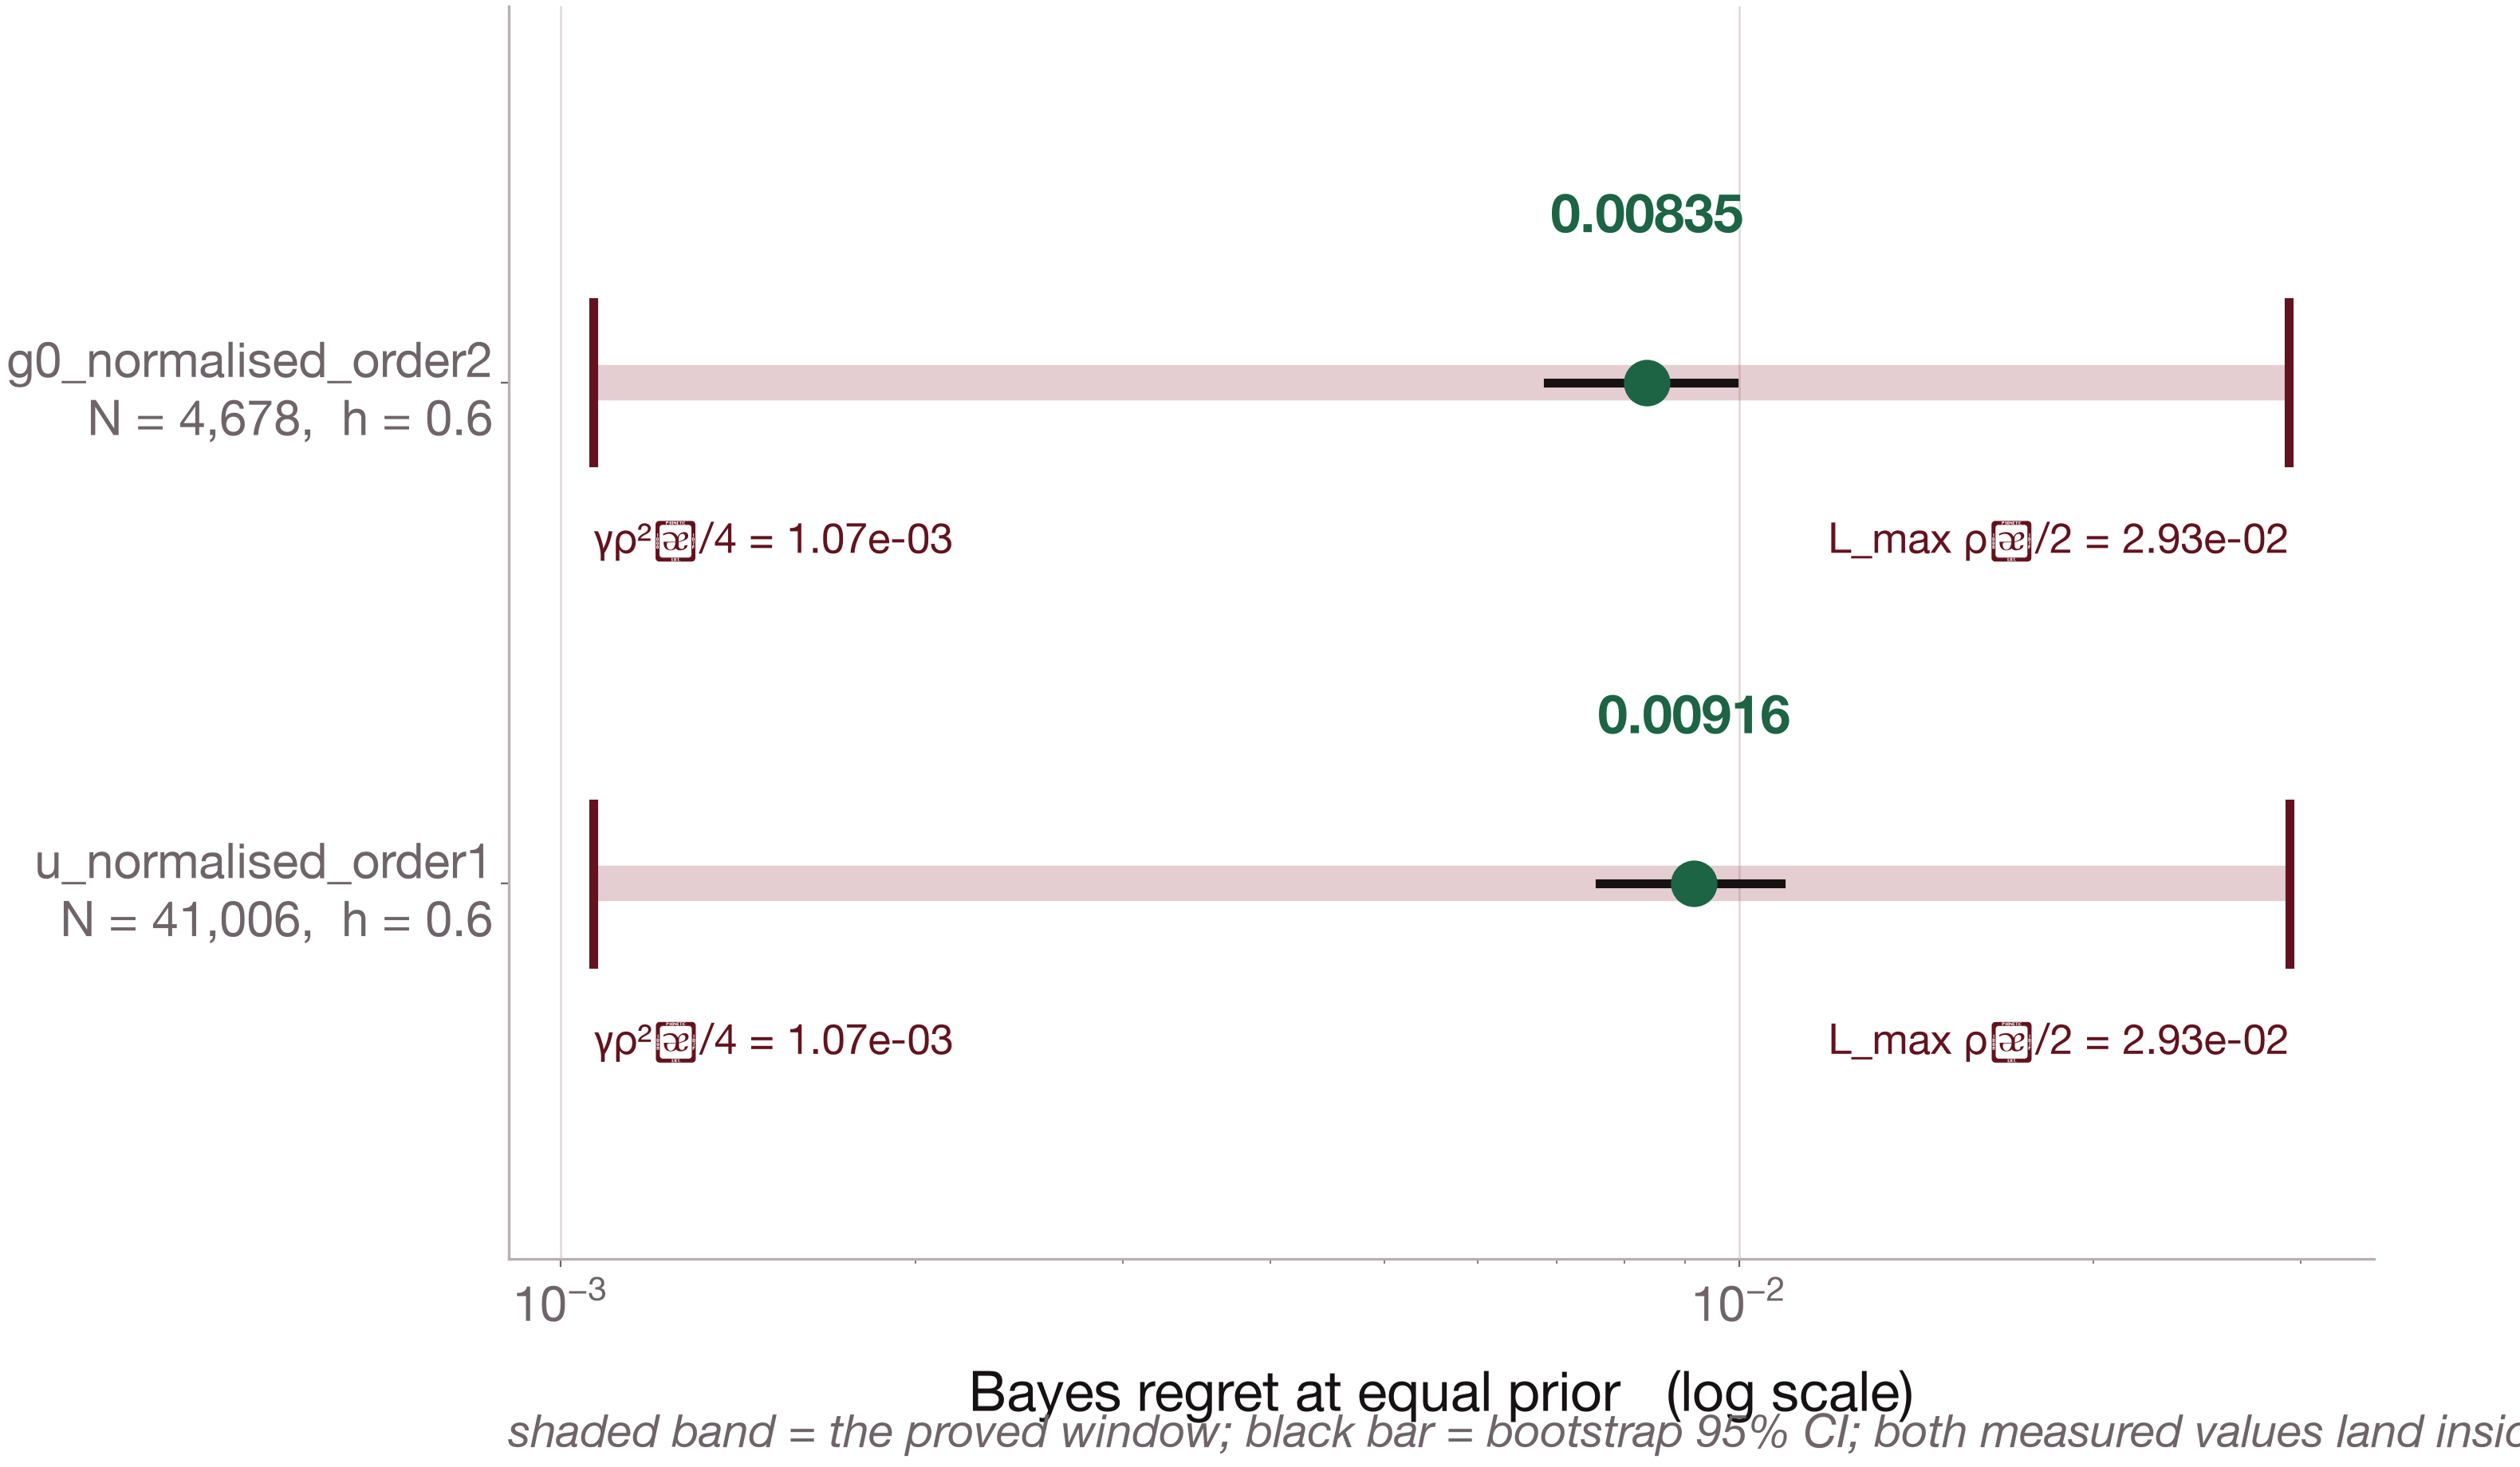
\includegraphics[width=\columnwidth]{query_fig1_regret.png}
\caption{Measured Bayes regret against the proved window of Theorem~\ref{thm:regret} for
two admissible measurements of the same worlds. The shaded band is the window; the black
bar is a percentile bootstrap $95\%$ interval over $2000$ resamples. The order-$1$
measurement needs almost nine times as many samples as the order-$2$ measurement to reach
the same error, although the worlds it is discriminating are identical.}
\label{fig:regret}
\end{figure}

\begin{table*}[t]
\caption{Full simulation record for the two admissible measurements of
Section~\ref{sec:experiments}. The two worlds are identical across both measurements; only
$g$ differs. Regret is measured per world and then combined under an equal prior, and the
percentile bootstrap uses 2000 resamples. The proved window is
$[\frac{\gamma}{4}\rho^{2N},\,\frac{L_{\max}}{2}\rho^{N}]$ from Theorem~\ref{thm:regret}
with $\gamma=13983/32768$ and $L_{\max}=2401/4096$, both exact rationals. Every measured value lies strictly
inside its window, and no bootstrap interval crosses either end.}
\label{tab:fullquery}
\centering
\footnotesize
\setlength{\tabcolsep}{5pt}
\begin{tabular}{@{}llrrrrlr@{}}
\toprule
Measurement & World & $h$ & per-sample $H^{2}$ & $N$ & error rate & mean regret & s.e. \\
\midrule
\lean{g0\_normalised\_order2} & 0 & 0.6 & 4.922e-04 & 4,678 & 0.0150 & 0.008793 & 0.001127 \\
\lean{g0\_normalised\_order2} & 1 & 0.6 & 4.922e-04 & 4,678 & 0.0135 & 0.007913 & 0.001070 \\
\multicolumn{2}{@{}l}{\emph{equal prior}} & & & & & 0.008353 & \\
\multicolumn{2}{@{}l}{\emph{bootstrap CI95}} & & & & & [0.006888,\,0.009892] & \\
\multicolumn{2}{@{}l}{\emph{proved window}} & & & & & [0.001066,\,0.029298] & inside \\
\midrule
\lean{u\_normalised\_order1} & 0 & 0.6 & 5.615e-05 & 41,006 & 0.0155 & 0.009086 & 0.001145 \\
\lean{u\_normalised\_order1} & 1 & 0.6 & 5.615e-05 & 41,006 & 0.0158 & 0.009232 & 0.001154 \\
\multicolumn{2}{@{}l}{\emph{equal prior}} & & & & & 0.009159 & \\
\multicolumn{2}{@{}l}{\emph{bootstrap CI95}} & & & & & [0.007620,\,0.010844] & \\
\multicolumn{2}{@{}l}{\emph{proved window}} & & & & & [0.001067,\,0.029308] & inside \\
\bottomrule
\end{tabular}
\end{table*}


\subsection{Reading the factor 8.8}

The factor is not a constant of the problem; it is $h^{-2(r_{1}-r_{2})}$ up to the explicit
constants of Theorem~\ref{thm:sandwich}, with $r_{1}-r_{2}=1$ and $h=0.6$ here. Halving $h$
would roughly quadruple it. This is the operational content of ``the order is a property of
the query'': the penalty for the wrong measurement is not additive and does not wash out
with more data---it is an exponent, and it compounds as the regime gets harder.

\section{The constants}
\label{sec:constants}

Theorem~\ref{thm:sandwich} contains two constants, and their status differs.

\subsection{$a_{E}$, and why it is instance-specific}

The lower constant arises from an interval $E$ and a bound $|\Delta_{r}|\ge a_{E}$ on it.
Theorem~\ref{thm:nonvanish} guarantees such a pair exists---a continuous function that is
not identically zero is bounded away from zero on some interval---but it does not produce
the best one, and the best one depends on the instance. Taking $E$ larger increases the
measure entering the Cauchy--Schwarz step but decreases the achievable $a_{E}$; the product
$a_{E}^{2}|E|^{2}$ is what the bound actually depends on, and optimising it is a
one-dimensional problem on the instance.

For the comparison of Section~\ref{sec:experiments} this optimisation is unnecessary,
because the two measurements are compared through their exact per-sample $H^{2}$ rather than
through the envelope. The constant matters only when the envelope itself is to be used as a
prediction, which is a stronger use than the paper makes of it.

\subsection{$J$, and what makes it finite}

The upper constant is the integral of the squared order-$r$ coefficient against the
reference density,
\begin{equation}
J \;=\; \int \frac{\Delta_{r}^{2}}{p_{0}} ,
\end{equation}
the same quantity that appears in the limit \eqref{eq:limit} up to the factor $8$. Its
finiteness is not automatic: $\Delta_{r}$ is a polynomial times a Gaussian and $p_{0}$ is a
mixture of Gaussians, so the ratio is a polynomial times a ratio of Gaussians, and the
latter can grow. What controls it is that every level appearing in $\Delta_{r}$ also
appears in $p_{0}$---again the shared-level-set hypothesis---so the growing exponential is
dominated. This is the integrable envelope that the upper side of
Theorem~\ref{thm:sandwich} and the dominated convergence of Theorem~\ref{thm:limit} both
consume, and it is constructed rather than assumed.

\subsection{Why the two constants are reported rather than absorbed}

It would be shorter to state Theorem~\ref{thm:sandwich} as
$H^{2}\asymp h^{2r}$. That form is adequate for an asymptotic claim and inadequate for the
paper's actual use, which is a comparison between two measurements at a \emph{fixed}
$h=0.6$. At fixed $h$ an unquantified $\asymp$ permits the two envelopes to be separated by
any factor whatever, and the observed ratio $8.8$ could then be attributed entirely to
constants rather than to the order. Writing both constants down is what makes the
attribution in C1 checkable.

\section{A worked instance}
\label{sec:instance}

The abstract statements are easier to trust against a concrete case, so we record the one
the experiments use.

The response takes values in a finite set of levels; the perturbation $g$ redistributes
mixture weight among them. For the order-$2$ measurement, the level coefficients
$M_{1}(v)$ cancel identically across levels---each level's contribution at order $1$ is
matched by another's---so $\Delta_{1}\equiv0$ and the order is at least $2$. At order $2$
the cancellation fails at the top level: the largest level carrying weight has
$c_{v^{*}}\neq0$ and is strictly largest, so Theorem~\ref{thm:nonvanish} applies and
$r=2$ exactly.

For the order-$1$ measurement, the same two worlds are probed by a different $g$ under
which the order-$1$ coefficients do \emph{not} cancel, so $r=1$. Note the direction: the
order-$1$ measurement is the \emph{worse} one. A smaller leakage order means the difference
between the worlds appears at a lower power of $h$ in the \emph{coefficient} indexing, and
in this parameterisation that corresponds to the smaller Hellinger distance---
$5.62\times10^{-5}$ against $4.92\times10^{-4}$---hence the larger sample requirement. The
numbers in Table~\ref{tab:query} are computed from \eqref{eq:mixture} directly, with no
appeal to the sandwich, which is what makes their position inside the window a check on the
sandwich rather than a consequence of it.

\section{Determining the order of a candidate query}
\label{sec:procedure}

The results above are worth little to a designer who cannot tell, given a candidate
measurement, what order it has. The proofs supply a procedure, and it is finite.

\begin{enumerate}
\item \textbf{Enumerate the levels.} Collect the distinct values $v$ taken by the response
$f_{W}$ over the mixture index set, together with the aggregate weight sitting at each.
\item \textbf{Form the level coefficients.} For $j=0,1,2,\dots$ compute $M_{j}(v)$ by
grouping the $j$-th order terms of the expansion of \eqref{eq:mixture} by level. By
Theorem~\ref{thm:sumswap} this is a finite sum, so the computation is exact.
\item \textbf{Test cancellation.} If every $M_{j}(v)$ vanishes, or if the non-zero ones
cancel across levels, increment $j$. This is the half handled by
\lean{mixture\_coeff\_diff\_eq\_zero}.
\item \textbf{Check the top level.} At the first $j$ where cancellation fails, identify the
largest level $v^{*}$ with $M_{j}(v^{*})\neq0$. If it is strictly largest,
Theorem~\ref{thm:nonvanish} certifies $r=j$ and the procedure terminates. If it ties with
another level, the procedure returns ``undetermined'': this case is outside the theorem and
is reported rather than guessed.
\item \textbf{Read the cost.} With $r$ in hand, Theorem~\ref{thm:sandwich} brackets
$H^{2}$, Theorem~\ref{thm:samples} converts the bracket into a sample count, and
Theorem~\ref{thm:regret} into a regret window.
\end{enumerate}

Two properties of this procedure are worth noting. It never requires simulating the
measurement: steps 1--4 are exact arithmetic on the mixture data, so a designer can
compare candidate queries before collecting any data. And step~4 has an explicit failure
mode rather than a silent one---the tie case is reported as undetermined, which is the
honest output given that Theorem~\ref{thm:nonvanish} does not cover it.

\subsection{What the procedure costs}

Steps 1--3 are linear in the number of mixture components per order examined, and the
number of orders examined is $r+1$. There is no search and no optimisation. The expensive
part in practice is not the order determination but the constants $a_{E}$ and $J$ of
Theorem~\ref{thm:sandwich}, which require an interval on which $|\Delta_{r}|$ is bounded
below and an integrable envelope respectively; both are constructive but instance-specific.
For the comparison in Section~\ref{sec:experiments} the orders alone were sufficient,
because the two measurements differ by one in $r$ and the $h^{-2}$ factor dominates any
ratio of constants at $h=0.6$.

\section{Formal verification}
\label{sec:verification}

Every theorem above is machine-checked in Lean~4, toolchain
\texttt{leanprover/lean4:v4.34.0-rc2} against mathlib revision \texttt{1f495c61}.

\subsection{Acceptance contract}

A module counts as accepted only when all six of the following hold: the compiler exits
zero with no errors; the source hash is unchanged \emph{across} the compile, so the file
checked is the file on disk; the compiled artifact is newer than its source; at least one
\texttt{\#print axioms} directive is present; the axiom set of every audited declaration
lies within $\{\textsf{propext},\textsf{Classical.choice},\textsf{Quot.sound}\}$; and no
\texttt{sorry} appears anywhere in the file.

\subsection{The crux statements as they are checked}

\begin{figure}[htbp]
\footnotesize
\hrule\vspace{4pt}
\begin{tabbing}
\quad\=\quad\=\kill
\lean{theorem levelSum\_ne\_zero ($\sigma$ : $\mathbb{R}$) (h$\sigma$ : $\sigma$ $\ne$ 0)} \\
\> \lean{(r : $\mathbb{N}$) (S : Finset $\mathbb{R}$) (c : $\mathbb{R}$ $\to$ $\mathbb{R}$) (vstar : $\mathbb{R}$)} \\
\> \lean{(hvs : vstar $\in$ S)} \\
\> \lean{(htop : $\forall$ v $\in$ S, v $\ne$ vstar $\to$ v < vstar)} \\
\> \lean{(hc : c vstar $\ne$ 0) :} \\
\> \lean{$\exists$ y, levelSum $\sigma$ r S c y $\ne$ 0} \\[6pt]
\lean{theorem mixture\_coeff\_ne\_zero ($\sigma$ : $\mathbb{R}$) (h$\sigma$ : $\sigma$ $\ne$ 0)} \\
\> \lean{(pi f g : X $\to$ $\mathbb{R}$) (r : $\mathbb{N}$) (vstar : $\mathbb{R}$)} \\
\> \lean{(hvs : vstar $\in$ Finset.image f univ)} \\
\> \lean{(htop : $\forall$ v $\in$ Finset.image f univ,} \\
\> \qquad\lean{v $\ne$ vstar $\to$ v < vstar)} \\
\> \lean{(hc : levelMoment pi f g r vstar $\ne$ 0) :} \\
\> \lean{$\exists$ y, iteratedDeriv r} \\
\> \qquad\lean{(fun h $\Rightarrow$ $\sum$ x, pi x * gauss $\sigma$ (y - f x - h * g x)) 0 $\ne$ 0}
\end{tabbing}
\vspace{-4pt}\hrule
\caption{The non-vanishing theorem and its mixture form, reproduced as the prover has them.
The hypothesis \lean{htop} is the strict top level of Remark~2; \lean{hc} is the non-zero
coefficient there. Both are quantified over an arbitrary finite level set, an arbitrary
coefficient function, and---in the mixture form---arbitrary weights \lean{pi}, response
\lean{f} and perturbation \lean{g}, so nothing is assumed about how the configuration
arose.}
\label{fig:statements}
\end{figure}

The conclusion is \lean{$\exists$ y, $\ldots$ $\ne$ 0}, which is exactly
$\Delta_{r}\not\equiv0$: a function is not identically zero precisely when it is non-zero
somewhere. That is the form the leakage order \eqref{eq:order} needs, and it is weaker than
it may look in one respect worth stating---it produces \emph{a} point where the coefficient
survives, not a set of positive measure. The lower side of
Theorem~\ref{thm:sandwich} needs an interval, and it obtains one from this point by
continuity, which is a step the paper carries out rather than a Lean statement.

The companion \lean{mixture\_coeff\_diff\_eq\_zero} supplies the other half of
\eqref{eq:order}---that the coefficients below order $r$ cancel---with the shared level set
appearing as an explicit hypothesis \lean{hS} and the agreeing moments as \lean{hagree}.
The two together justify the definition rather than only its non-degeneracy.

\subsection{Evidence per step}

\begin{table}[htbp]
\caption{Evidence per step of the chain. All cited declarations are axiom-audited.}
\label{tab:inventory}
\centering
\footnotesize
\setlength{\tabcolsep}{3pt}
\begin{tabular}{@{}llr@{}}
\toprule
Step & Module & Aud. \\
\midrule
Derivatives, Thm~\ref{thm:hermite}   & \lean{LeanQueryGaussianLevelV1}     & 13 \\
Sum rule, Thm~\ref{thm:sumswap}      & \lean{LeanQueryMixtureDerivativeV1} &  5 \\
Non-vanishing, Thm~\ref{thm:nonvanish} & \lean{LeanQueryGaussianLevelV1}   & 18 \\
                                     & \lean{LeanQueryMixtureDerivativeV1} &    \\
Sandwich, Thm~\ref{thm:sandwich}     & \lean{LeanQueryHellingerIntervalV1} & 14 \\
                                     & \lean{LeanQueryTaylorRemainderV1}   &    \\
Per-sample, Lem~\ref{lem:logsandwich}& \lean{LeanQuerySampleComplexityV1}  &  8 \\
Sample counts, Thm~\ref{thm:samples} & \lean{LeanQuerySampleComplexityV1}  &  8 \\
Regret, Thm~\ref{thm:regret}         & \lean{LeanQueryRegretBridgeV1}      &  5 \\
Limit, Thm~\ref{thm:limit}           & \lean{LeanQueryAnalyticLimitV1}     &  4 \\
\bottomrule
\end{tabular}
\end{table}

\subsection{What formalisation caught}

Three defects in earlier drafts of this chain were found by the prover rather than by
reading, and they are recorded because they indicate what the discipline is worth on a
problem of this shape.

The lower constant in Theorem~\ref{thm:sandwich} was initially $16$. The step producing it
bounded $(\sqrt{p}+\sqrt{q})^{2}$ by $p+q$, which is false---the correct bound is
$2(p+q)$---and the error is invisible in a numerical check, because the resulting envelope
is still a valid lower bound on any instance where the slack absorbs the factor. The prover
refused the step.

The smoothness hypothesis in Theorem~\ref{thm:sumswap} was initially assumed. Mathlib's
multilinear sum rule requires $C^{\infty}$ of each summand, and the mixture components are
$C^{\infty}$ only because $\exp$ composed with a polynomial is; stating that as an
assumption would have left the paper's main technical contribution resting on an unproved
side condition. It is now derived.

The non-vanishing argument originally used the largest level without requiring it to be
\emph{strictly} largest. With a tie, the two exponential factors have identical decay and
the limit argument in Theorem~\ref{thm:nonvanish} produces $0=0$ rather than a
contradiction. The hypothesis \lean{htop} in Fig.~\ref{fig:statements} is the repair, and
the tie case is now reported as out of scope in Remark~2 rather than silently assumed away.

\subsection{Scope of the formalisation}

The displayed results are the load-bearing chain, not the corpus. The Query strand contains
$27$ Lean source files with $167$ theorem and lemma statements, of which $13$ modules carry
an acceptance receipt covering $87$ declarations whose axiom set was printed and checked.
Across the programme of which this paper is one part: $762$ files, $7{,}199$ statements,
$111$ accepted modules, $875$ audited declarations.

No module cited in this paper contains a \texttt{sorry}. Seven occurrences exist in the
wider repository, in audit scaffolding and in files named as conjectures; the overlap
between the cited set and the files containing them was computed and is empty.

The statements not displayed are the machinery the displayed ones stand on: arithmetic
lemmas, measurability side conditions, finite-sum exchanges, and the counterexamples that
ruled out earlier formulations of the sandwich---including one in which the lower constant
was taken to be $16$, which the prover rejected.

\subsection{Reproducibility}

The simulation is deterministic given its seed. Each row of Table~\ref{tab:fullquery} is
$4000$ independent repetitions per world at the stated $N$, with the decision rule being the
likelihood-ratio test that Theorem~\ref{thm:regret}'s upper side analyses; the regret is the
realised loss minus the loss of the best fixed action, averaged, and the equal-prior figure
is the mean of the two per-world means. The bootstrap is a percentile bootstrap over the
$8000$ per-repetition regrets with $2000$ resamples.

The quantities entering the window---$\gamma$, $L_{\max}$, and $\rho=1-H^{2}$---are computed
in exact rational arithmetic where the loss geometry permits ($\gamma=13983/32768$,
$L_{\max}=2401/4096$) and in double precision otherwise. The window endpoints in
Table~\ref{tab:fullquery} are therefore reproducible to the last digit shown, and the
measured regrets to within the reported standard errors.

\section{Discussion}
\label{sec:discussion}

\subsection{What the results establish}

The result reframes what an experimenter controls. Where the parameter space is fixed by
nature, the measurement class is often a design choice, and the leakage order---hence the
exponent of the rate---moves with it. Theorem~\ref{thm:nonvanish} is what licenses the
reframing: without it a vanishing order-$r$ coefficient would leave the order undefined and
the comparison between queries meaningless. Theorem~\ref{thm:limit} then certifies that the
constant in front of the rate is real, so the comparison is between two genuine leading
terms rather than between two envelopes.

\subsection{What the results do not establish}

\begin{enumerate}
\item \textbf{Normalisation.} Constants $1/(\sigma\sqrt{2\pi})$ and $1/j!$ are dropped
throughout. The dropped expressions must not be quoted as densities.

\item \textbf{A shared level set.} The cancellation statement assumes the two worlds share a
level set. Worlds whose responses have disjoint level structure are outside it.

\item \textbf{A strict top level.} Theorem~\ref{thm:nonvanish} needs the largest level
carrying a non-zero coefficient to be strictly largest. Ties at the top are not covered, and
no claim is made about them.

\item \textbf{A window, not a value.} The ends of \eqref{eq:regret} separate as $N$ grows,
so the result localises regret without determining it.

\item \textbf{No minimax statement.} Nothing here is a statement about the worst case over
a class of worlds or of measurements. Every result is about a fixed pair and a fixed query.
\end{enumerate}

\subsection{Why the comparison is fair}

An objection to C1 would be that the two measurements differ in more than their order---in
their noise scale, say, or their effective sample size per observation---so that
attributing the factor $8.8$ to the order is overreach. Three features of the design close
that objection. The worlds $f_{0},f_{1}$ are byte-identical across the two runs, so the
parameter space is fixed by construction. The noise $\sigma$ and the perturbation scale
$h=0.6$ are shared, so the per-observation cost is the same. And the per-sample $H^{2}$ is
computed directly from \eqref{eq:mixture} in both cases rather than through the sandwich,
so the reported $4.92\times10^{-4}$ and $5.62\times10^{-5}$ are properties of the
measurements themselves.

What remains is the sample count, and it is determined by $H^{2}$ through
Theorem~\ref{thm:samples} with no free parameter. The comparison therefore isolates exactly
one difference---which $g$ was legal---and reports its price.

\subsection{Limitations of the simulation}

Three limitations of Section~\ref{sec:experiments} are worth naming, none of which affects
the theorems.

The comparison uses two measurements, not a family. A sweep over many $g$ would show the
order's effect as a curve rather than as two points, and would let the $h$-dependence of the
factor be measured rather than predicted. It was not run, and the factor $8.8$ should be
read as one instance of the prediction $h^{-2(r_{1}-r_{2})}$ up to constants rather than as
a fitted exponent.

The scale $h=0.6$ is not small. The asymptotic statements hold as $h\downarrow0$, and at
$0.6$ the remainder terms suppressed in Theorem~\ref{thm:sandwich} are not negligible. This
is why the per-sample $H^{2}$ is computed exactly from \eqref{eq:mixture} rather than from
the envelope; the envelope is used only to place the measured regret inside a window, which
it does with room to spare in both rows of Table~\ref{tab:fullquery}.

The regret window is wide. Its ends differ by a factor of roughly $27$ on the order-$2$
row, which reflects the $\rho^{2N}$ against $\rho^{N}$ gap of Theorem~\ref{thm:regret}
rather than any looseness in the measurement. A measured value inside such a window is a
consistency check, not a sharp test, and it is reported as such.

\subsection{Open problems}

Closing the regret window---replacing \eqref{eq:regret} by a two-sided bound whose ends
agree to a constant factor uniformly in $N$---is the first question, and it appears to need
a sharper handle on the likelihood-ratio test's error than the affinity supplies. The tied
top level is the second: when two levels share the maximum, the exponential factors in
Theorem~\ref{thm:nonvanish} no longer separate, and whether non-vanishing survives is open.
Third, the map from a measurement to its leakage order is currently computed case by case;
a criterion reading $r$ off $g$ and the level structure directly would turn the design
question into a calculation. Finally, the limit in Theorem~\ref{thm:limit} is identified as
an integral but not evaluated in closed form for any non-trivial family.

\subsection{Where the framing applies}

The pattern the paper isolates is not specific to Gaussian mixtures. It requires only that
the observation law admit an expansion in a perturbation scale whose coefficients depend on
the measurement, and that the first non-vanishing coefficient control a divergence. Where
those hold, the same three questions arise: whether the cancellation below the claimed
order is genuine, whether the coefficient at that order really fails to vanish, and whether
the resulting envelope has a positive limit. The middle question is the one this paper
argues should not be assumed, and the tie case of Remark~2 is a concrete reminder that the
assumption can fail.

Conversely, the framing has no content where the measurement class is a single element---
where the experimenter observes what nature provides and cannot choose---which is the
setting of most of the mixture-rate literature. The contribution is therefore
complementary to that work rather than competing with it: the same expansion machinery, run
with the roles of the fixed and the variable object exchanged.

\section{Conclusion}

The leakage order is a property of the query, not of the parameter space, and the chain
establishing this is closed end to end and machine-checked: Gaussian derivatives built
explicitly, the derivative pushed through the finite sum, the order-$r$ coefficient proved
not to vanish, $H^{2}$ sandwiched with explicit constants of matching exponent, converted
into matching sample counts, bracketed as regret, and finally shown to converge with a
strictly positive limit. On an instance where the worlds are held fixed, changing which
measurement is legal changes the sample requirement by a factor of $8.8$, and that factor
is an exponent in $h$ rather than a constant.

For a practitioner the summary is short. Before choosing a measurement, enumerate its
levels and find the first order at which the coefficients fail to cancel; check that the
top level carrying weight there is strictly largest; and if it is, the sample requirement
scales as $h^{-2r}$ with that $r$. If two candidate measurements differ by one in $r$, the
cheaper one is cheaper by a factor of order $h^{-2}$, and no amount of additional data from
the expensive one recovers the difference---it is an exponent, not a constant.

\appendices
\section{Complete statement inventory}
\label{app:inventory}

The Query strand contributes $87$ axiom-audited theorems and lemmas across its accepted modules. Those that any step of this paper uses are displayed in Section~\ref{sec:setting}, beside the step that consumes them. This appendix reproduces the \emph{complete} chain---every audited statement of the strand, grouped by module, including the ones already shown---so that the development can be read end to end without reassembling it from the body.

Each entry is a symbol-level transliteration of the Lean statement: Unicode maps to the corresponding \LaTeX{} symbol and identifiers are set upright, but no structure is rewritten and no hypothesis is dropped. Binders are listed as the prover has them and the turnstile $\vdash$ separates them from the conclusion. Every entry carries an acceptance receipt and an axiom audit confining it to $\{\textsf{propext},\textsf{Classical.choice},\textsf{Quot.sound}\}$; none contains \texttt{sorry}.

\vspace{4pt}\noindent\rule{\columnwidth}{0.4pt}\par\vspace{2pt}
\noindent\textbf{Module \lean{LeanQueryAffinityTestingV1}}\par\vspace{3pt}

\noindent\textbf{A\,1}\quad\lean{affinity\_enclosure}
{\footnotesize\[ \begin{aligned}[t]
&(\mathit{rho} \mathit{hlo} \mathit{hhi} : \mathbb{R}\\
&\quad ),\; (\mathit{hlo\_{}bound} : \mathit{hlo} \leq 1-\mathit{rho}),\;\\
&\quad (\mathit{hhi\_{}bound} : 1-\mathit{rho} \leq \mathit{hhi})
\end{aligned} \]}
{\footnotesize\[ \begin{aligned}[t]
\vdash\;&1-\mathit{hhi} \leq \mathit{rho}\\
&\quad \wedge \mathit{rho} \leq 1-\mathit{hlo}
\end{aligned} \]}

\noindent\textbf{A\,2}\quad\lean{every\_test\_lower}
{\footnotesize\[ \begin{aligned}[t]
&(\mu : \mathit{Measure} \Omega ),\; (\mathit{p}\\
&\quad \mathit{q} \mathit{d} : \Omega \to \mathbb{R}\\
&\quad ),\; (\mathit{hd0} : \forall \mathit{x}, 0 \leq \mathit{d}\\
&\quad \mathit{x}),\; (\mathit{hd1} : \forall \mathit{x},\\
&\quad \mathit{d} \mathit{x} \leq 1),\; (\mathit{imin} :\\
&\quad \mathit{Integrable} (\mathbf{fun} \mathit{x} =>\\
&\quad \mathit{min} (\mathit{p} \mathit{x}) (\mathit{q}\\
&\quad \mathit{x})) \mu ),\; (\mathit{iloss} :\\
&\quad \mathit{Integrable} (\mathbf{fun} \mathit{x} =>\\
&\quad \mathit{p} \mathit{x}*\mathit{d} \mathit{x}+\mathit{q}\\
&\quad \mathit{x}*(1-\mathit{d} \mathit{x})) \mu )
\end{aligned} \]}
{\footnotesize\[ \begin{aligned}[t]
\vdash\;&\mathit{overlap} \mu \mathit{p}\\
&\quad \mathit{q}/2 \leq \mathit{testingError}\\
&\quad \mu \mathit{p} \mathit{q} \mathit{d}
\end{aligned} \]}

\noindent\textbf{A\,3}\quad\lean{iid\_affinity}
{\footnotesize\[ \begin{aligned}[t]
&(\mu : \mathit{Measure} \Omega ),\;\\
&\quad [\mathit{SigmaFinite} \mu ],\; (\mathit{p} \mathit{q}\\
&\quad : \Omega \to \mathbb{R} ),\; (\mathit{hp} : \forall \mathit{x},\\
&\quad 0 \leq \mathit{p} \mathit{x}),\; (\mathit{hq} :\\
&\quad \forall \mathit{x}, 0 \leq \mathit{q}\\
&\quad \mathit{x}),\; (\mathit{N} : \mathbb{N}\\
&\quad )
\end{aligned} \]}
{\footnotesize\[ \begin{aligned}[t]
\vdash\;&\mathit{affinity} (\mathit{Measure}.\mathit{pi}\\
&\quad (\mathbf{fun} \mathit{\_{}} : \mathit{Fin} \mathit{N}\\
&\quad => \mu )) (\mathit{iidDensity} \mathit{p}\\
&\quad \mathit{N}) (\mathit{iidDensity} \mathit{q}\\
&\quad \mathit{N}) = (\mathit{affinity} \mu \mathit{p}\\
&\quad \mathit{q})^{\mathit{N}}
\end{aligned} \]}

\noindent\textbf{A\,4}\quad\lean{iid\_normalized}
{\footnotesize\[ \begin{aligned}[t]
&(\mu : \mathit{Measure} \Omega ),\;\\
&\quad [\mathit{SigmaFinite} \mu ],\; (\mathit{p} : \Omega \to \mathbb{R}\\
&\quad ),\; (\mathit{hp} : \int \mathit{x}, \mathit{p}\\
&\quad \mathit{x} ∂\mu = 1),\; (\mathit{N} : \mathbb{N}\\
&\quad )
\end{aligned} \]}
{\footnotesize\[ \begin{aligned}[t]
\vdash\;&(\int \mathit{x}, \mathit{iidDensity} \mathit{p}\\
&\quad \mathit{N} \mathit{x} ∂\mathit{Measure}.\mathit{pi}\\
&\quad (\mathbf{fun} \mathit{\_{}} : \mathit{Fin} \mathit{N}\\
&\quad => \mu )) = 1
\end{aligned} \]}

\noindent\textbf{A\,5}\quad\lean{iid\_testing\_bracket}
{\footnotesize\[ \begin{aligned}[t]
&(\mu : \mathit{Measure} \Omega ),\;\\
&\quad [\mathit{SigmaFinite} \mu ],\; (\mathit{p} \mathit{q}\\
&\quad : \Omega \to \mathbb{R} ),\; (\mathit{hp} : \forall \mathit{x},\\
&\quad 0 \leq \mathit{p} \mathit{x}),\; (\mathit{hq} :\\
&\quad \forall \mathit{x}, 0 \leq \mathit{q}\\
&\quad \mathit{x}),\; (\mathit{np} : \int \mathit{x},\\
&\quad \mathit{p} \mathit{x} ∂\mu = 1),\; (\mathit{nq} : \int \mathit{x},\\
&\quad \mathit{q} \mathit{x} ∂\mu = 1),\; (\mathit{N} :\\
&\quad \mathbb{N} ),\; (\mathit{ip} : \mathit{Integrable}\\
&\quad (\mathit{iidDensity} \mathit{p} \mathit{N})\\
&\quad (\mathit{Measure}.\mathit{pi} (\mathbf{fun}\\
&\quad \mathit{\_{}} : \mathit{Fin} \mathit{N} => \mu ))),\;\\
&\quad (\mathit{iq} : \mathit{Integrable}\\
&\quad (\mathit{iidDensity} \mathit{q} \mathit{N})\\
&\quad (\mathit{Measure}.\mathit{pi} (\mathbf{fun}\\
&\quad \mathit{\_{}} : \mathit{Fin} \mathit{N} => \mu ))),\;\\
&\quad (\mathit{imin} : \mathit{Integrable} (\mathbf{fun}\\
&\quad \mathit{x} => \mathit{min} (\mathit{iidDensity}\\
&\quad \mathit{p} \mathit{N} \mathit{x}) (\mathit{iidDensity}\\
&\quad \mathit{q} \mathit{N} \mathit{x}))\\
&\quad (\mathit{Measure}.\mathit{pi} (\mathbf{fun}\\
&\quad \mathit{\_{}} : \mathit{Fin} \mathit{N} => \mu ))),\;\\
&\quad (\mathit{iroot} : \mathit{Integrable} (\mathbf{fun}\\
&\quad \mathit{x} => \mathit{Real}.\mathit{sqrt}\\
&\quad (\mathit{iidDensity} \mathit{p} \mathit{N}\\
&\quad \mathit{x}*\mathit{iidDensity} \mathit{q} \mathit{N}\\
&\quad \mathit{x})) (\mathit{Measure}.\mathit{pi}\\
&\quad (\mathbf{fun} \mathit{\_{}} : \mathit{Fin} \mathit{N}\\
&\quad => \mu )))
\end{aligned} \]}
{\footnotesize\[ \begin{aligned}[t]
\vdash\;&(\mathit{affinity} \mu \mathit{p}\\
&\quad \mathit{q})^{}(2*\mathit{N})/4\\
&\quad \leq \mathit{testingError}\\
&\quad (\mathit{Measure}.\mathit{pi} (\mathbf{fun}\\
&\quad \mathit{\_{}} : \mathit{Fin} \mathit{N} => \mu ))\\
&\quad (\mathit{iidDensity} \mathit{p}\\
&\quad \mathit{N}) (\mathit{iidDensity} \mathit{q}\\
&\quad \mathit{N}) (\mathit{likelihoodRatioTest}\\
&\quad (\mathit{iidDensity} \mathit{p} \mathit{N})\\
&\quad (\mathit{iidDensity} \mathit{q}\\
&\quad \mathit{N})) \wedge \mathit{testingError}\\
&\quad (\mathit{Measure}.\mathit{pi} (\mathbf{fun}\\
&\quad \mathit{\_{}} : \mathit{Fin} \mathit{N} => \mu ))\\
&\quad (\mathit{iidDensity} \mathit{p}\\
&\quad \mathit{N}) (\mathit{iidDensity} \mathit{q}\\
&\quad \mathit{N}) (\mathit{likelihoodRatioTest}\\
&\quad (\mathit{iidDensity} \mathit{p} \mathit{N})\\
&\quad (\mathit{iidDensity} \mathit{q}\\
&\quad \mathit{N})) \leq (\mathit{affinity} \mu \mathit{p}\\
&\quad \mathit{q})^{\mathit{N}}/2
\end{aligned} \]}

\noindent\textbf{A\,6}\quad\lean{likelihood\_ratio\_attains}
{\footnotesize\[ \begin{aligned}[t]
&(\mu : \mathit{Measure} \Omega ),\; (\mathit{p}\\
&\quad \mathit{q} : \Omega \to \mathbb{R} )
\end{aligned} \]}
{\footnotesize\[ \begin{aligned}[t]
\vdash\;&\mathit{testingError} \mu \mathit{p}\\
&\quad \mathit{q} (\mathit{likelihoodRatioTest} \mathit{p}\\
&\quad \mathit{q}) = \mathit{overlap} \mu \mathit{p}\\
&\quad \mathit{q}/2
\end{aligned} \]}

\noindent\textbf{A\,7}\quad\lean{min\_le\_root}
{\footnotesize\[ \begin{aligned}[t]
&(\mathit{p} \mathit{q} : \mathbb{R}\\
&\quad ),\; (\mathit{hp} : 0 \leq \mathit{p}),\; (\mathit{hq}\\
&\quad : 0 \leq \mathit{q})
\end{aligned} \]}
{\footnotesize\[ \begin{aligned}[t]
\vdash\;&\mathit{min} \mathit{p} \mathit{q}\\
&\quad \leq \mathit{Real}.\mathit{sqrt}\\
&\quad (\mathit{p}*\mathit{q})
\end{aligned} \]}

\noindent\textbf{A\,8}\quad\lean{overlap\_bracket}
{\footnotesize\[ \begin{aligned}[t]
&(\mu : \mathit{Measure} \Omega ),\; (\mathit{p}\\
&\quad \mathit{q} : \Omega \to \mathbb{R} ),\; (\mathit{hp} :\\
&\quad \forall \mathit{x}, 0 \leq \mathit{p}\\
&\quad \mathit{x}),\; (\mathit{hq} : \forall \mathit{x}, 0\\
&\quad \leq \mathit{q} \mathit{x}),\; (\mathit{ip} :\\
&\quad \mathit{Integrable} \mathit{p} \mu ),\; (\mathit{iq} :\\
&\quad \mathit{Integrable} \mathit{q} \mu ),\; (\mathit{imin}\\
&\quad : \mathit{Integrable} (\mathbf{fun} \mathit{x} =>\\
&\quad \mathit{min} (\mathit{p} \mathit{x}) (\mathit{q}\\
&\quad \mathit{x})) \mu ),\; (\mathit{iroot} :\\
&\quad \mathit{Integrable} (\mathbf{fun} \mathit{x} =>\\
&\quad \mathit{Real}.\mathit{sqrt} (\mathit{p}\\
&\quad \mathit{x}*\mathit{q} \mathit{x})) \mu ),\;\\
&\quad (\mathit{np} : \int \mathit{x}, \mathit{p} \mathit{x}\\
&\quad ∂\mu = 1),\; (\mathit{nq} : \int \mathit{x},\\
&\quad \mathit{q} \mathit{x} ∂\mu = 1)
\end{aligned} \]}
{\footnotesize\[ \begin{aligned}[t]
\vdash\;&(\mathit{affinity} \mu \mathit{p}\\
&\quad \mathit{q})^{2}/4 \leq \mathit{overlap}\\
&\quad \mu \mathit{p} \mathit{q}/2 \wedge \mathit{overlap}\\
&\quad \mu \mathit{p} \mathit{q}/2 \leq \mathit{affinity}\\
&\quad \mu \mathit{p} \mathit{q}/2
\end{aligned} \]}

\noindent\textbf{A\,9}\quad\lean{root\_young}
{\footnotesize\[ \begin{aligned}[t]
&(\mathit{p} \mathit{q} \mathit{t} : \mathbb{R}\\
&\quad ),\; (\mathit{hp} : 0 \leq \mathit{p}),\; (\mathit{hq}\\
&\quad : 0 \leq \mathit{q})
\end{aligned} \]}
{\footnotesize\[ \begin{aligned}[t]
\vdash\;&2*\mathit{t}*\mathit{Real}.\mathit{sqrt}\\
&\quad (\mathit{p}*\mathit{q}) \leq \mathit{min}\\
&\quad \mathit{p} \mathit{q} +\\
&\quad \mathit{t}^{2}*(\mathit{p}+\mathit{q})
\end{aligned} \]}

\vspace{4pt}\noindent\rule{\columnwidth}{0.4pt}\par\vspace{2pt}
\noindent\textbf{Module \lean{LeanQueryAnalyticLimitV1}}\par\vspace{3pt}

\noindent\textbf{A\,10}\quad\lean{eventually\_pos\_of\_limit\_pos}
{\footnotesize\[ \begin{aligned}[t]
&(\mathit{H2} : \mathbb{R} \to \mathbb{R}\\
&\quad ),\; (\mathit{L} : \mathbb{R} ),\; (\mathit{hL} : 0 <\\
&\quad \mathit{L}),\; (\mathit{hlim} : \mathit{Tendsto}\\
&\quad \mathit{H2} (𝓝[>] (0:\mathbb{R} )) (𝓝\\
&\quad \mathit{L}))
\end{aligned} \]}
{\footnotesize\[ \begin{aligned}[t]
\vdash\;&\forall ᶠ \mathit{h} \mathbf{in} 𝓝[>] (0:\mathbb{R}\\
&\quad ), 0 < \mathit{H2} \mathit{h}
\end{aligned} \]}

\noindent\textbf{A\,11}\quad\lean{hellinger\_ratio\_tendsto}
{\footnotesize\[ \begin{aligned}[t]
&(\mu : \mathit{Measure} \Omega ),\; (\mathit{F} :\\
&\quad \mathbb{R} \to \Omega \to \mathbb{R}\\
&\quad ),\; (\mathit{Dr} \mathit{p0} \mathit{bound} : \Omega \to \mathbb{R}\\
&\quad ),\; (\mathit{H2} : \mathbb{R} \to \mathbb{R}\\
&\quad ),\; (\mathit{hmeas} : \forall ᶠ \mathit{h}\\
&\quad \mathbf{in} 𝓝[>] (0:\mathbb{R} ),\\
&\quad \mathit{AEStronglyMeasurable} (\mathit{F} \mathit{h})\\
&\quad \mu ),\; (\mathit{hdom} : \forall ᶠ \mathit{h}\\
&\quad \mathbf{in} 𝓝[>] (0:\mathbb{R} ), \forall ᵐ \mathit{x}\\
&\quad ∂\mu , \Vert \mathit{F} \mathit{h} \mathit{x}\Vert \leq \mathit{bound}\\
&\quad \mathit{x}),\; (\mathit{hint} : \mathit{Integrable}\\
&\quad \mathit{bound} \mu ),\; (\mathit{hptw} : \forall ᵐ\\
&\quad \mathit{x} ∂\mu , \mathit{Tendsto} (\mathbf{fun}\\
&\quad \mathit{h} => \mathit{F} \mathit{h} \mathit{x}) (𝓝[>]\\
&\quad (0:\mathbb{R} )) (𝓝 (\mathit{Dr} \mathit{x} ^{2} / (4\\
&\quad * \mathit{p0} \mathit{x})))),\; (\mathit{hH2} :\\
&\quad \forall \mathit{h} : \mathbb{R} , \mathit{H2}\\
&\quad \mathit{h} = (1/2) * \int \mathit{x}, \mathit{F}\\
&\quad \mathit{h} \mathit{x} ∂\mu )
\end{aligned} \]}
{\footnotesize\[ \begin{aligned}[t]
\vdash\;&\mathit{Tendsto} \mathit{H2} (𝓝[>] (0:\mathbb{R}\\
&\quad )) (𝓝 ((1/2) * \int \mathit{x}, \mathit{Dr} \mathit{x}\\
&\quad ^{2} / (4 * \mathit{p0} \mathit{x}) ∂\mu ))
\end{aligned} \]}

\noindent\textbf{A\,12}\quad\lean{limit\_pos\_of\_ae\_ne\_zero}
{\footnotesize\[ \begin{aligned}[t]
&(\mu : \mathit{Measure} \Omega ),\; (\mathit{g} :\\
&\quad \Omega \to \mathbb{R} ),\; (\mathit{hnn} : 0 \leq ᵐ[\mu ]\\
&\quad \mathit{g}),\; (\mathit{hint} : \mathit{Integrable}\\
&\quad \mathit{g} \mu ),\; (\mathit{hne} : \neg (\mathit{g}\\
&\quad =ᵐ[\mu ] 0))
\end{aligned} \]}
{\footnotesize\[ \begin{aligned}[t]
\vdash\;&0 < \int \mathit{x}, \mathit{g}\\
&\quad \mathit{x} ∂\mu
\end{aligned} \]}

\noindent\textbf{A\,13}\quad\lean{ratio\_tendsto\_of\_dominated}
{\footnotesize\[ \begin{aligned}[t]
&(\mu : \mathit{Measure} \Omega ),\; (\mathit{F} :\\
&\quad \mathbb{R} \to \Omega \to \mathbb{R}\\
&\quad ),\; (\mathit{lim} \mathit{bound} : \Omega \to \mathbb{R}\\
&\quad ),\; (\mathit{hmeas} : \forall ᶠ \mathit{h}\\
&\quad \mathbf{in} 𝓝[>] (0:\mathbb{R} ),\\
&\quad \mathit{AEStronglyMeasurable} (\mathit{F} \mathit{h})\\
&\quad \mu ),\; (\mathit{hdom} : \forall ᶠ \mathit{h}\\
&\quad \mathbf{in} 𝓝[>] (0:\mathbb{R} ), \forall ᵐ \mathit{x}\\
&\quad ∂\mu , \Vert \mathit{F} \mathit{h} \mathit{x}\Vert \leq \mathit{bound}\\
&\quad \mathit{x}),\; (\mathit{hint} : \mathit{Integrable}\\
&\quad \mathit{bound} \mu ),\; (\mathit{hptw} : \forall ᵐ\\
&\quad \mathit{x} ∂\mu , \mathit{Tendsto} (\mathbf{fun}\\
&\quad \mathit{h} => \mathit{F} \mathit{h} \mathit{x}) (𝓝[>]\\
&\quad (0:\mathbb{R} )) (𝓝 (\mathit{lim}\\
&\quad \mathit{x})))
\end{aligned} \]}
{\footnotesize\[ \begin{aligned}[t]
\vdash\;&\mathit{Tendsto} (\mathbf{fun} \mathit{h} => \int \mathit{x},\\
&\quad \mathit{F} \mathit{h} \mathit{x} ∂\mu ) (𝓝[>]\\
&\quad (0:\mathbb{R} )) (𝓝 (\int \mathit{x}, \mathit{lim}\\
&\quad \mathit{x} ∂\mu ))
\end{aligned} \]}

\vspace{4pt}\noindent\rule{\columnwidth}{0.4pt}\par\vspace{2pt}
\noindent\textbf{Module \lean{LeanQueryCriticalResolutionV1}}\par\vspace{3pt}

\noindent\textbf{A\,14}\quad\lean{at\_critical\_fails}
{\footnotesize\[ \begin{aligned}[t]
&(\mathit{R} : \Theta \to \mathit{D} \to \mathbb{R}\\
&\quad ),\; (\mathit{g} : \Theta \to \mathbb{R}\\
&\quad ),\; (\mathit{eps} : \mathbb{R} ),\; (\mathit{hn} :\\
&\quad (\mathit{badPairs} \mathit{g}\\
&\quad \mathit{eps}).\mathit{Nonempty})
\end{aligned} \]}
{\footnotesize\[ \begin{aligned}[t]
\vdash\;&\mathit{eps} \notin \mathit{feasibleErrors}\\
&\quad \mathit{R} \mathit{g} (\mathit{critical} \mathit{R}\\
&\quad \mathit{g} \mathit{eps} \mathit{hn})
\end{aligned} \]}

\noindent\textbf{A\,15}\quad\lean{below\_critical\_sufficient}
{\footnotesize\[ \begin{aligned}[t]
&(\mathit{R} : \Theta \to \mathit{D} \to \mathbb{R}\\
&\quad ),\; (\mathit{g} : \Theta \to \mathbb{R}\\
&\quad ),\; (\mathit{eta} \mathit{eps} : \mathbb{R}\\
&\quad ),\; (\mathit{he} : 0 \leq \mathit{eta}),\;\\
&\quad (\mathit{hn} : (\mathit{badPairs} \mathit{g}\\
&\quad \mathit{eps}).\mathit{Nonempty}),\; (\mathit{hlt} :\\
&\quad \mathit{eta}<\mathit{critical} \mathit{R} \mathit{g}\\
&\quad \mathit{eps} \mathit{hn})
\end{aligned} \]}
{\footnotesize\[ \begin{aligned}[t]
\vdash\;&\mathit{eps} \in \mathit{feasibleErrors}\\
&\quad \mathit{R} \mathit{g} \mathit{eta}
\end{aligned} \]}

\noindent\textbf{A\,16}\quad\lean{critical\_nonneg}
{\footnotesize\[ \begin{aligned}[t]
&(\mathit{R} : \Theta \to \mathit{D} \to \mathbb{R}\\
&\quad ),\; (\mathit{g} : \Theta \to \mathbb{R}\\
&\quad ),\; (\mathit{eps} : \mathbb{R} ),\; (\mathit{hn} :\\
&\quad (\mathit{badPairs} \mathit{g}\\
&\quad \mathit{eps}).\mathit{Nonempty})
\end{aligned} \]}
{\footnotesize\[ \begin{aligned}[t]
\vdash\;&0 \leq \mathit{critical} \mathit{R}\\
&\quad \mathit{g} \mathit{eps} \mathit{hn}
\end{aligned} \]}

\noindent\textbf{A\,17}\quad\lean{feasible\_iff\_pair\_bound}
{\footnotesize\[ \begin{aligned}[t]
&(\mathit{R} : \Theta \to \mathit{D} \to \mathbb{R}\\
&\quad ),\; (\mathit{g} : \Theta \to \mathbb{R}\\
&\quad ),\; (\mathit{eta} \mathit{eps} : \mathbb{R}\\
&\quad ),\; (\mathit{he} : 0 \leq \mathit{eta})
\end{aligned} \]}
{\footnotesize\[ \begin{aligned}[t]
\vdash\;&\mathit{eps} \in \mathit{feasibleErrors}\\
&\quad \mathit{R} \mathit{g} \mathit{eta}\\
&\quad \leftrightarrow \forall \mathit{x}\\
&\quad \mathit{z},\mathit{Close} \mathit{R}\\
&\quad \mathit{eta} \mathit{x} \mathit{z}\\
&\quad \to |\mathit{g} \mathit{x}-\mathit{g}\\
&\quad \mathit{z}| \leq 2*\mathit{eps}
\end{aligned} \]}

\noindent\textbf{A\,18}\quad\lean{no\_bad\_pairs\_sufficient}
{\footnotesize\[ \begin{aligned}[t]
&(\mathit{R} : \Theta \to \mathit{D} \to \mathbb{R}\\
&\quad ),\; (\mathit{g} : \Theta \to \mathbb{R}\\
&\quad ),\; (\mathit{eta} \mathit{eps} : \mathbb{R}\\
&\quad ),\; (\mathit{he} : 0 \leq \mathit{eta}),\;\\
&\quad (\mathit{hn} : \mathit{badPairs} \mathit{g}\\
&\quad \mathit{eps}=\emptyset )
\end{aligned} \]}
{\footnotesize\[ \begin{aligned}[t]
\vdash\;&\mathit{eps} \in \mathit{feasibleErrors}\\
&\quad \mathit{R} \mathit{g} \mathit{eta}
\end{aligned} \]}

\vspace{4pt}\noindent\rule{\columnwidth}{0.4pt}\par\vspace{2pt}
\noindent\textbf{Module \lean{LeanQueryGaussianLevelV1}}\par\vspace{3pt}

\noindent\textbf{A\,19}\quad\lean{gauss\_pos}
{\footnotesize\[ \begin{aligned}[t]
&(\sigma \mathit{y} : \mathbb{R} )
\end{aligned} \]}
{\footnotesize\[ \begin{aligned}[t]
\vdash\;&0 < \mathit{gauss} \sigma \mathit{y}
\end{aligned} \]}

\noindent\textbf{A\,20}\quad\lean{gauss\_shift}
{\footnotesize\[ \begin{aligned}[t]
&(\sigma : \mathbb{R} ),\; (\mathit{hσ} : \sigma \neq 0),\;\\
&\quad (\mathit{v} \mathit{y} : \mathbb{R} )
\end{aligned} \]}
{\footnotesize\[ \begin{aligned}[t]
\vdash\;&\mathit{gauss} \sigma (\mathit{y} -\\
&\quad \mathit{v}) = \mathit{gauss} \sigma \mathit{y}\\
&\quad * \mathit{Real}.\mathit{exp} (\mathit{v} * \mathit{y}\\
&\quad / \sigma ^{2} - \mathit{v} ^{2} / (2 * \sigma ^{2}))
\end{aligned} \]}

\noindent\textbf{A\,21}\quad\lean{hasDerivAt\_gauss}
{\footnotesize\[ \begin{aligned}[t]
&(\sigma : \mathbb{R} ),\; (\mathit{hσ} : \sigma \neq 0),\;\\
&\quad (\mathit{y} : \mathbb{R} )
\end{aligned} \]}
{\footnotesize\[ \begin{aligned}[t]
\vdash\;&\mathit{HasDerivAt} (\mathit{gauss} \sigma )\\
&\quad (-(\mathit{y} / \sigma ^{2}) * \mathit{gauss} \sigma \mathit{y})\\
&\quad \mathit{y}
\end{aligned} \]}

\noindent\textbf{A\,22}\quad\lean{hasDerivAt\_hgauss}
{\footnotesize\[ \begin{aligned}[t]
&(\sigma : \mathbb{R} ),\; (\mathit{hσ} : \sigma \neq 0),\;\\
&\quad (\mathit{j} : \mathbb{N} ),\; (\mathit{z} : \mathbb{R}\\
&\quad )
\end{aligned} \]}
{\footnotesize\[ \begin{aligned}[t]
\vdash\;&\mathit{HasDerivAt} (\mathbf{fun} \mathit{w} =>\\
&\quad (\mathit{hpoly} \sigma \mathit{j}).\mathit{eval}\\
&\quad \mathit{w} * \mathit{gauss} \sigma \mathit{w})\\
&\quad ((\mathit{hpoly} \sigma (\mathit{j} +\\
&\quad 1)).\mathit{eval} \mathit{z} * \mathit{gauss} \sigma \mathit{z})\\
&\quad \mathit{z}
\end{aligned} \]}

\noindent\textbf{A\,23}\quad\lean{hpoly\_coeff}
{\footnotesize\[ \begin{aligned}[t]
&(\sigma : \mathbb{R} )
\end{aligned} \]}
{\footnotesize\[ \begin{aligned}[t]
\vdash\;&\forall \mathit{n} : \mathbb{N} , (\mathit{hpoly}\\
&\quad \sigma \mathit{n}).\mathit{coeff}\\
&\quad \mathit{n} = (-(1 / \sigma ^{2}))\\
&\quad ^{\mathit{n}}
\end{aligned} \]}

\noindent\textbf{A\,24}\quad\lean{hpoly\_natDegree\_le}
{\footnotesize\[ \begin{aligned}[t]
&(\sigma : \mathbb{R} )
\end{aligned} \]}
{\footnotesize\[ \begin{aligned}[t]
\vdash\;&\forall \mathit{n} : \mathbb{N} , (\mathit{hpoly}\\
&\quad \sigma \mathit{n}).\mathit{natDegree}\\
&\quad \leq \mathit{n}
\end{aligned} \]}

\noindent\textbf{A\,25}\quad\lean{hpoly\_ne\_zero}
{\footnotesize\[ \begin{aligned}[t]
&(\sigma : \mathbb{R} ),\; (\mathit{hσ} : \sigma \neq 0),\;\\
&\quad (\mathit{n} : \mathbb{N} )
\end{aligned} \]}
{\footnotesize\[ \begin{aligned}[t]
\vdash\;&\mathit{hpoly} \sigma \mathit{n}\\
&\quad \neq 0
\end{aligned} \]}

\noindent\textbf{A\,26}\quad\lean{iteratedDeriv\_gauss}
{\footnotesize\[ \begin{aligned}[t]
&(\sigma : \mathbb{R} ),\; (\mathit{hσ} : \sigma \neq 0)
\end{aligned} \]}
{\footnotesize\[ \begin{aligned}[t]
\vdash\;&\forall (\mathit{n} : \mathbb{N} ) (\mathit{y} :\\
&\quad \mathbb{R} ), \mathit{iteratedDeriv}\\
&\quad \mathit{n} (\mathit{gauss} \sigma )\\
&\quad \mathit{y} = (\mathit{hpoly} \sigma \mathit{n}).\mathit{eval}\\
&\quad \mathit{y} * \mathit{gauss} \sigma \mathit{y}
\end{aligned} \]}

\noindent\textbf{A\,27}\quad\lean{iteratedDeriv\_shift}
{\footnotesize\[ \begin{aligned}[t]
&(\sigma : \mathbb{R} ),\; (\mathit{hσ} : \sigma \neq 0),\;\\
&\quad (\mathit{g} \mathit{v} \mathit{y} : \mathbb{R}\\
&\quad )
\end{aligned} \]}
{\footnotesize\[ \begin{aligned}[t]
\vdash\;&\forall (\mathit{j} : \mathbb{N} ) (\mathit{h₀} :\\
&\quad \mathbb{R} ), \mathit{iteratedDeriv}\\
&\quad \mathit{j} (\mathbf{fun} \mathit{h} : \mathbb{R} =>\\
&\quad \mathit{gauss} \sigma (\mathit{y} - \mathit{v} -\\
&\quad \mathit{h} * \mathit{g})) \mathit{h₀}\\
&\quad = (-\mathit{g}) ^{\mathit{j}} * ((\mathit{hpoly}\\
&\quad \sigma \mathit{j}).\mathit{eval} (\mathit{y} -\\
&\quad \mathit{v} - \mathit{h₀} * \mathit{g}) *\\
&\quad \mathit{gauss} \sigma (\mathit{y} - \mathit{v} -\\
&\quad \mathit{h₀} * \mathit{g}))
\end{aligned} \]}

\noindent\textbf{A\,28}\quad\lean{levelSum\_eq\_zero\_of\_levels\_agree}
{\footnotesize\[ \begin{aligned}[t]
&(\sigma : \mathbb{R} ),\; (\mathit{r} : \mathbb{N}\\
&\quad ),\; (\mathit{S} : \mathit{Finset} \mathbb{R}\\
&\quad ),\; (\mathit{cA} \mathit{cB} : \mathbb{R} \to \mathbb{R}\\
&\quad ),\; (\mathit{hagree} : \forall \mathit{v} \in \mathit{S},\\
&\quad \mathit{cA} \mathit{v} = \mathit{cB}\\
&\quad \mathit{v}),\; (\mathit{y} : \mathbb{R}\\
&\quad )
\end{aligned} \]}
{\footnotesize\[ \begin{aligned}[t]
\vdash\;&\mathit{levelSum} \sigma \mathit{r}\\
&\quad \mathit{S} \mathit{cA} \mathit{y} -\\
&\quad \mathit{levelSum} \sigma \mathit{r}\\
&\quad \mathit{S} \mathit{cB} \mathit{y}\\
&\quad = 0
\end{aligned} \]}

\noindent\textbf{A\,29}\quad\lean{levelSum\_ne\_zero}
{\footnotesize\[ \begin{aligned}[t]
&(\sigma : \mathbb{R} ),\; (\mathit{hσ} : \sigma \neq 0),\;\\
&\quad (\mathit{r} : \mathbb{N} ),\; (\mathit{S} :\\
&\quad \mathit{Finset} \mathbb{R} ),\; (\mathit{c} :\\
&\quad \mathbb{R} \to \mathbb{R} ),\; (\mathit{vstar} :\\
&\quad \mathbb{R} ),\; (\mathit{hvs} : \mathit{vstar} \in \mathit{S}),\;\\
&\quad (\mathit{htop} : \forall \mathit{v} \in \mathit{S},\\
&\quad \mathit{v} \neq \mathit{vstar} \to \mathit{v} <\\
&\quad \mathit{vstar}),\; (\mathit{hc} : \mathit{c}\\
&\quad \mathit{vstar} \neq 0)
\end{aligned} \]}
{\footnotesize\[ \begin{aligned}[t]
\vdash\;&\exists \mathit{y}, \mathit{levelSum}\\
&\quad \sigma \mathit{r} \mathit{S} \mathit{c}\\
&\quad \mathit{y} \neq 0
\end{aligned} \]}

\noindent\textbf{A\,30}\quad\lean{poly\_exp\_decay}
{\footnotesize\[ \begin{aligned}[t]
&(\mathit{p} : \mathbb{R}\\
&\quad [\mathit{X}]),\; (\mathit{v} \delta : \mathbb{R}\\
&\quad ),\; (\mathit{hδ} : 0 < \delta )
\end{aligned} \]}
{\footnotesize\[ \begin{aligned}[t]
\vdash\;&\mathit{Tendsto} (\mathbf{fun} \mathit{y} : \mathbb{R}\\
&\quad => \mathit{p}.\mathit{eval} (\mathit{y} - \mathit{v})\\
&\quad * \mathit{Real}.\mathit{exp} (-(\delta *\\
&\quad \mathit{y}))) \mathit{atTop} (𝓝 0)
\end{aligned} \]}

\noindent\textbf{A\,31}\quad\lean{sum\_by\_level}
{\footnotesize\[ \begin{aligned}[t]
&\{ \mathit{X} : \mathit{Type}*\},\; [\mathit{Fintype}\\
&\quad \mathit{X}],\; [\mathit{DecidableEq}\\
&\quad \mathit{X}],\; (\mathit{pi} \mathit{f} \mathit{w} :\\
&\quad \mathit{X} \to \mathbb{R} ),\; (\mathit{Q} :\\
&\quad \mathbb{R} \to \mathbb{R} )
\end{aligned} \]}
{\footnotesize\[ \begin{aligned}[t]
\vdash\;&\textstyle\sum \mathit{x} : \mathit{X},\\
&\quad \mathit{pi} \mathit{x} * \mathit{w}\\
&\quad \mathit{x} * \mathit{Q} (\mathit{f}\\
&\quad \mathit{x}) = \textstyle\sum \mathit{v}\\
&\quad \in \mathit{Finset}.\mathit{image}\\
&\quad \mathit{f}\\
&\quad \mathit{Finset}.\mathit{univ}, (\textstyle\sum \mathit{x}\\
&\quad \in \mathit{Finset}.\mathit{univ}.\mathit{filter}\\
&\quad (\mathbf{fun} \mathit{x} => \mathit{f} \mathit{x} =\\
&\quad \mathit{v}), \mathit{pi} \mathit{x} * \mathit{w}\\
&\quad \mathit{x}) * \mathit{Q} \mathit{v}
\end{aligned} \]}

\vspace{4pt}\noindent\rule{\columnwidth}{0.4pt}\par\vspace{2pt}
\noindent\textbf{Module \lean{LeanQueryHellingerEnvelopeV1}}\par\vspace{3pt}

\noindent\textbf{A\,32}\quad\lean{chi2\_pointwise}
{\footnotesize\[ \begin{aligned}[t]
&(\mathit{p} \mathit{q} : \mathbb{R}\\
&\quad ),\; (\mathit{hp} : 0 \leq \mathit{p}),\; (\mathit{hq}\\
&\quad : 0 < \mathit{q})
\end{aligned} \]}
{\footnotesize\[ \begin{aligned}[t]
\vdash\;&(\mathit{Real}.\mathit{sqrt} \mathit{p} -\\
&\quad \mathit{Real}.\mathit{sqrt} \mathit{q})\\
&\quad ^{2} \leq (\mathit{p} - \mathit{q})\\
&\quad ^{2} / \mathit{q}
\end{aligned} \]}

\noindent\textbf{A\,33}\quad\lean{envelope\_bound}
{\footnotesize\[ \begin{aligned}[t]
&(\mathit{C0} \mathit{C1} \mathit{b} : \mathbb{R}\\
&\quad ),\; (\mathit{r} : \mathbb{N} ),\; (\mathit{y} :\\
&\quad \mathbb{R} ),\; (\mathit{hb} : 0 <\\
&\quad \mathit{b}),\; (\mathit{hC0} : 0 \leq \mathit{C0}),\;\\
&\quad (\mathit{hC1} : 0 \leq \mathit{C1})
\end{aligned} \]}
{\footnotesize\[ \begin{aligned}[t]
\vdash\;&(\mathit{C0} + \mathit{C1} * (\mathit{y} ^{2})\\
&\quad ^{\mathit{r}}) *\\
&\quad \mathit{Real}.\mathit{exp} (-(\mathit{b} * \mathit{y}\\
&\quad ^{2})) \leq \mathit{C0} *\\
&\quad \mathit{Real}.\mathit{exp} (-(\mathit{b} / 2 *\\
&\quad \mathit{y} ^{2})) + \mathit{C1} * (((2 * (\mathit{r} :\\
&\quad \mathbb{R} )) / \mathit{b}) ^{\mathit{r}} *\\
&\quad \mathit{Real}.\mathit{exp} (-(\mathit{b} / 2 *\\
&\quad \mathit{y} ^{2})))
\end{aligned} \]}

\noindent\textbf{A\,34}\quad\lean{envelope\_integrable}
{\footnotesize\[ \begin{aligned}[t]
&(\mathit{C0} \mathit{C1} \mathit{b} : \mathbb{R}\\
&\quad ),\; (\mathit{r} : \mathbb{N} ),\; (\mathit{hb} : 0 <\\
&\quad \mathit{b}),\; (\mathit{hC0} : 0 \leq \mathit{C0}),\;\\
&\quad (\mathit{hC1} : 0 \leq \mathit{C1})
\end{aligned} \]}
{\footnotesize\[ \begin{aligned}[t]
\vdash\;&\mathit{Integrable} (\mathbf{fun} \mathit{y} :\\
&\quad \mathbb{R} => (\mathit{C0} + \mathit{C1} * (\mathit{y}\\
&\quad ^{2}) ^{\mathit{r}}) * \mathit{Real}.\mathit{exp}\\
&\quad (-(\mathit{b} * \mathit{y} ^{2})))
\end{aligned} \]}

\noindent\textbf{A\,35}\quad\lean{gauss\_lower\_envelope}
{\footnotesize\[ \begin{aligned}[t]
&(\sigma \mathit{M} \mathit{m} \mathit{y} : \mathbb{R}\\
&\quad ),\; (\mathit{hσ} : 0 < \sigma ),\; (\mathit{hm} :\\
&\quad |\mathit{m}| \leq \mathit{M})
\end{aligned} \]}
{\footnotesize\[ \begin{aligned}[t]
\vdash\;&\mathit{Real}.\mathit{exp} (-(\mathit{y} ^{2}) / (2 *\\
&\quad \sigma ^{2}) - \mathit{M} * |\mathit{y}| / \sigma ^{2}\\
&\quad - \mathit{M} ^{2} / (2 * \sigma ^{2}))\\
&\quad \leq \mathit{Real}.\mathit{exp} (-((\mathit{y} -\\
&\quad \mathit{m}) ^{2}) / (2 * \sigma ^{2}))
\end{aligned} \]}

\noindent\textbf{A\,36}\quad\lean{gauss\_upper\_envelope}
{\footnotesize\[ \begin{aligned}[t]
&(\sigma \mathit{M} \mathit{m} \mathit{y} : \mathbb{R}\\
&\quad ),\; (\mathit{hσ} : 0 < \sigma ),\; (\mathit{hm} :\\
&\quad |\mathit{m}| \leq \mathit{M})
\end{aligned} \]}
{\footnotesize\[ \begin{aligned}[t]
\vdash\;&\mathit{Real}.\mathit{exp} (-((\mathit{y} -\\
&\quad \mathit{m}) ^{2}) / (2 * \sigma ^{2}))\\
&\quad \leq \mathit{Real}.\mathit{exp} (-(\mathit{y} ^{2}) /\\
&\quad (2 * \sigma ^{2}) + \mathit{M} * |\mathit{y}| / \sigma ^{2})
\end{aligned} \]}

\noindent\textbf{A\,37}\quad\lean{majorise}
{\footnotesize\[ \begin{aligned}[t]
&(\mathit{M} \mathit{y} : \mathbb{R} )
\end{aligned} \]}
{\footnotesize\[ \begin{aligned}[t]
\vdash\;&3 * \mathit{M} * |\mathit{y}| \leq \mathit{y}\\
&\quad ^{2} / 4 + 9 * \mathit{M} ^{2}
\end{aligned} \]}

\noindent\textbf{A\,38}\quad\lean{mixture\_ge\_component}
{\footnotesize\[ \begin{aligned}[t]
&\{ \mathit{X} : \mathit{Type}*\},\; [\mathit{Fintype}\\
&\quad \mathit{X}],\; [\mathit{DecidableEq}\\
&\quad \mathit{X}],\; (\mathit{pi} \mathit{f} : \mathit{X}\\
&\quad \to \mathbb{R} ),\; (\mathit{hpi} : \forall \mathit{x},\\
&\quad 0 \leq \mathit{pi} \mathit{x}),\; (\mathit{hf} :\\
&\quad \forall \mathit{x}, 0 \leq \mathit{f}\\
&\quad \mathit{x}),\; (\mathit{x₀} :\\
&\quad \mathit{X})
\end{aligned} \]}
{\footnotesize\[ \begin{aligned}[t]
\vdash\;&\mathit{pi} \mathit{x₀} * \mathit{f}\\
&\quad \mathit{x₀} \leq \textstyle\sum \mathit{x},\\
&\quad \mathit{pi} \mathit{x} * \mathit{f}\\
&\quad \mathit{x}
\end{aligned} \]}

\noindent\textbf{A\,39}\quad\lean{pow\_le\_exp}
{\footnotesize\[ \begin{aligned}[t]
&(\mathit{n} : \mathbb{N} ),\; (\mathit{x} : \mathbb{R}\\
&\quad ),\; (\mathit{hx} : 0 \leq \mathit{x})
\end{aligned} \]}
{\footnotesize\[ \begin{aligned}[t]
\vdash\;&\mathit{x} ^{\mathit{n}} \leq (\mathit{n} : \mathbb{R}\\
&\quad ) ^{\mathit{n}} *\\
&\quad \mathit{Real}.\mathit{exp} \mathit{x}
\end{aligned} \]}

\noindent\textbf{A\,40}\quad\lean{sq\_pow\_le\_exp}
{\footnotesize\[ \begin{aligned}[t]
&(\mathit{r} : \mathbb{N} ),\; (\mathit{a} \mathit{y} :\\
&\quad \mathbb{R} ),\; (\mathit{ha} : 0 <\\
&\quad \mathit{a})
\end{aligned} \]}
{\footnotesize\[ \begin{aligned}[t]
\vdash\;&(\mathit{y} ^{2}) ^{\mathit{r}}\\
&\quad \leq ((\mathit{r} : \mathbb{R} ) /\\
&\quad \mathit{a}) ^{\mathit{r}} *\\
&\quad \mathit{Real}.\mathit{exp} (\mathit{a} * \mathit{y}\\
&\quad ^{2})
\end{aligned} \]}

\vspace{4pt}\noindent\rule{\columnwidth}{0.4pt}\par\vspace{2pt}
\noindent\textbf{Module \lean{LeanQueryHellingerIntervalV1}}\par\vspace{3pt}

\noindent\textbf{A\,41}\quad\lean{factor\_pointwise}
{\footnotesize\[ \begin{aligned}[t]
&(\mathit{p} \mathit{q} : \mathbb{R}\\
&\quad ),\; (\mathit{hp} : 0 \leq \mathit{p}),\; (\mathit{hq}\\
&\quad : 0 \leq \mathit{q})
\end{aligned} \]}
{\footnotesize\[ \begin{aligned}[t]
\vdash\;&\mathit{p} - \mathit{q} = (\mathit{Real}.\mathit{sqrt}\\
&\quad \mathit{p} - \mathit{Real}.\mathit{sqrt}\\
&\quad \mathit{q}) * (\mathit{Real}.\mathit{sqrt} \mathit{p}\\
&\quad + \mathit{Real}.\mathit{sqrt}\\
&\quad \mathit{q})
\end{aligned} \]}

\noindent\textbf{A\,42}\quad\lean{gap\_le\_of\_integrals}
{\footnotesize\[ \begin{aligned}[t]
&(\mu : \mathit{Measure} \Omega ),\; (\mathit{p}\\
&\quad \mathit{q} \mathit{chi} : \Omega \to \mathbb{R}\\
&\quad ),\; (\mathit{t} \mathit{H2} : \mathbb{R}\\
&\quad ),\; (\mathit{ht} : 0 < \mathit{t}),\; (\mathit{hp} :\\
&\quad \forall \mathit{x}, 0 \leq \mathit{p}\\
&\quad \mathit{x}),\; (\mathit{hq} : \forall \mathit{x}, 0\\
&\quad \leq \mathit{q} \mathit{x}),\; (\mathit{hchi0} :\\
&\quad \forall \mathit{x}, 0 \leq \mathit{chi}\\
&\quad \mathit{x}),\; (\mathit{hchi1} : \forall \mathit{x},\\
&\quad \mathit{chi} \mathit{x} \leq 1),\; (\mathit{hdiff} :\\
&\quad \mathit{Integrable} (\mathbf{fun} \mathit{x} =>\\
&\quad \mathit{chi} \mathit{x} * (\mathit{p} \mathit{x} -\\
&\quad \mathit{q} \mathit{x})) \mu ),\; (\mathit{hsq} :\\
&\quad \mathit{Integrable} (\mathbf{fun} \mathit{x} =>\\
&\quad (\mathit{Real}.\mathit{sqrt} (\mathit{p} \mathit{x}) -\\
&\quad \mathit{Real}.\mathit{sqrt} (\mathit{q} \mathit{x}))\\
&\quad ^{2}) \mu ),\; (\mathit{hsum} : \mathit{Integrable}\\
&\quad (\mathbf{fun} \mathit{x} =>\\
&\quad (\mathit{Real}.\mathit{sqrt} (\mathit{p} \mathit{x}) +\\
&\quad \mathit{Real}.\mathit{sqrt} (\mathit{q} \mathit{x}))\\
&\quad ^{2}) \mu ),\; (\mathit{hH2} : \int \mathit{x},\\
&\quad (\mathit{Real}.\mathit{sqrt} (\mathit{p} \mathit{x}) -\\
&\quad \mathit{Real}.\mathit{sqrt} (\mathit{q} \mathit{x}))\\
&\quad ^{2} ∂\mu = 2 * \mathit{H2}),\; (\mathit{hS} : \int \mathit{x},\\
&\quad (\mathit{Real}.\mathit{sqrt} (\mathit{p} \mathit{x}) +\\
&\quad \mathit{Real}.\mathit{sqrt} (\mathit{q} \mathit{x}))\\
&\quad ^{2} ∂\mu = 4 - 2 * \mathit{H2})
\end{aligned} \]}
{\footnotesize\[ \begin{aligned}[t]
\vdash\;&|\int \mathit{x}, \mathit{chi}\\
&\quad \mathit{x} * (\mathit{p} \mathit{x} - \mathit{q}\\
&\quad \mathit{x}) ∂\mu | \leq \mathit{t} *\\
&\quad \mathit{H2} + (4 - 2 * \mathit{H2}) / (2 *\\
&\quad \mathit{t})
\end{aligned} \]}

\noindent\textbf{A\,43}\quad\lean{hellinger\_lower\_from\_interval}
{\footnotesize\[ \begin{aligned}[t]
&(\mathit{H2} \mathit{aE} \mathit{hr} : \mathbb{R}\\
&\quad ),\; (\mathit{hH} : 0 \leq \mathit{H2}),\;\\
&\quad (\mathit{hr0} : 0 \leq \mathit{hr}),\;\\
&\quad (\mathit{hDbound} : \forall \mathit{t} : \mathbb{R} ,\\
&\quad 0 < \mathit{t} \to |\mathit{aE}| * \mathit{hr} / 2\\
&\quad \leq \mathit{t} * \mathit{H2} + 2 /\\
&\quad \mathit{t})
\end{aligned} \]}
{\footnotesize\[ \begin{aligned}[t]
\vdash\;&\mathit{aE} ^{2} * \mathit{hr} ^{2} /\\
&\quad 32 \leq \mathit{H2}
\end{aligned} \]}

\noindent\textbf{A\,44}\quad\lean{sq\_le\_of\_all\_t}
{\footnotesize\[ \begin{aligned}[t]
&(\mathit{D} \mathit{H2} : \mathbb{R}\\
&\quad ),\; (\mathit{hD} : 0 \leq \mathit{D}),\; (\mathit{hH}\\
&\quad : 0 \leq \mathit{H2}),\; (\mathit{hall} : \forall \mathit{t}\\
&\quad : \mathbb{R} , 0 < \mathit{t} \to \mathit{D} \leq \mathit{t}\\
&\quad * \mathit{H2} + 2 / \mathit{t})
\end{aligned} \]}
{\footnotesize\[ \begin{aligned}[t]
\vdash\;&\mathit{D} ^{2} \leq 8 * \mathit{H2}
\end{aligned} \]}

\noindent\textbf{A\,45}\quad\lean{sqrt\_sum\_sq\_identity}
{\footnotesize\[ \begin{aligned}[t]
&(\mathit{p} \mathit{q} : \mathbb{R}\\
&\quad ),\; (\mathit{hp} : 0 \leq \mathit{p}),\; (\mathit{hq}\\
&\quad : 0 \leq \mathit{q})
\end{aligned} \]}
{\footnotesize\[ \begin{aligned}[t]
\vdash\;&(\mathit{Real}.\mathit{sqrt} \mathit{p} +\\
&\quad \mathit{Real}.\mathit{sqrt} \mathit{q})\\
&\quad ^{2} = 2 * (\mathit{p} + \mathit{q}) -\\
&\quad (\mathit{Real}.\mathit{sqrt} \mathit{p} -\\
&\quad \mathit{Real}.\mathit{sqrt} \mathit{q})\\
&\quad ^{2}
\end{aligned} \]}

\noindent\textbf{A\,46}\quad\lean{sum\_sq\_integral}
{\footnotesize\[ \begin{aligned}[t]
&(\mu : \mathit{Measure} \Omega ),\; (\mathit{p}\\
&\quad \mathit{q} : \Omega \to \mathbb{R} ),\; (\mathit{H2} :\\
&\quad \mathbb{R} ),\; (\mathit{hp} : \forall \mathit{x}, 0\\
&\quad \leq \mathit{p} \mathit{x}),\; (\mathit{hq} : \forall \mathit{x},\\
&\quad 0 \leq \mathit{q} \mathit{x}),\; (\mathit{hpi} :\\
&\quad \mathit{Integrable} \mathit{p} \mu ),\; (\mathit{hqi}\\
&\quad : \mathit{Integrable} \mathit{q} \mu ),\;\\
&\quad (\mathit{hsq} : \mathit{Integrable} (\mathbf{fun}\\
&\quad \mathit{x} => (\mathit{Real}.\mathit{sqrt} (\mathit{p}\\
&\quad \mathit{x}) - \mathit{Real}.\mathit{sqrt} (\mathit{q}\\
&\quad \mathit{x})) ^{2}) \mu ),\; (\mathit{hH2} : \int \mathit{x},\\
&\quad (\mathit{Real}.\mathit{sqrt} (\mathit{p} \mathit{x}) -\\
&\quad \mathit{Real}.\mathit{sqrt} (\mathit{q} \mathit{x}))\\
&\quad ^{2} ∂\mu = 2 * \mathit{H2}),\; (\mathit{hpint} : \int \mathit{x},\\
&\quad \mathit{p} \mathit{x} ∂\mu = 1),\; (\mathit{hqint} :\\
&\quad \int \mathit{x}, \mathit{q} \mathit{x} ∂\mu =\\
&\quad 1)
\end{aligned} \]}
{\footnotesize\[ \begin{aligned}[t]
\vdash\;&\int \mathit{x}, (\mathit{Real}.\mathit{sqrt}\\
&\quad (\mathit{p} \mathit{x}) + \mathit{Real}.\mathit{sqrt}\\
&\quad (\mathit{q} \mathit{x})) ^{2} ∂\mu = 4\\
&\quad - 2 * \mathit{H2}
\end{aligned} \]}

\noindent\textbf{A\,47}\quad\lean{young\_pointwise}
{\footnotesize\[ \begin{aligned}[t]
&(\mathit{u} \mathit{v} \mathit{t} : \mathbb{R}\\
&\quad ),\; (\mathit{ht} : 0 < \mathit{t})
\end{aligned} \]}
{\footnotesize\[ \begin{aligned}[t]
\vdash\;&|\mathit{u} * \mathit{v}| \leq \mathit{t}\\
&\quad / 2 * \mathit{u} ^{2} + 1 / (2 *\\
&\quad \mathit{t}) * \mathit{v} ^{2}
\end{aligned} \]}

\vspace{4pt}\noindent\rule{\columnwidth}{0.4pt}\par\vspace{2pt}
\noindent\textbf{Module \lean{LeanQueryInterventionFloorV1}}\par\vspace{3pt}

\noindent\textbf{A\,48}\quad\lean{blind\_procedure\_floor}
{\footnotesize\[ \begin{aligned}[t]
&\{ \Omega : \mathit{Type}*\},\; [\mathit{Fintype}\\
&\quad \Omega ],\; (\mathit{mu} : \Omega \to \mathbb{R}\\
&\quad ),\; (\mathit{hmu} : \forall \mathit{o}, 0 \leq \mathit{mu}\\
&\quad \mathit{o}),\; (\mathit{hmus} : \textstyle\sum \mathit{o},\\
&\quad \mathit{mu} \mathit{o} = 1),\; (\mathit{rule} : \Omega \to \mathit{Dec}\\
&\quad \to \mathbb{R} ),\; (\mathit{hr} : \forall \mathit{o}\\
&\quad \mathit{S}, 0 \leq \mathit{rule} \mathit{o}\\
&\quad \mathit{S}),\; (\mathit{hrs} : \forall \mathit{o},\\
&\quad \textstyle\sum \mathit{S}, \mathit{rule} \mathit{o}\\
&\quad \mathit{S} = 1)
\end{aligned} \]}
{\footnotesize\[ \begin{aligned}[t]
\vdash\;&2401/8192 \leq \mathit{max} (\mathit{regretA}\\
&\quad (\mathbf{fun} \mathit{S} => \textstyle\sum \mathit{o},\\
&\quad \mathit{mu} \mathit{o}*\mathit{rule} \mathit{o}\\
&\quad \mathit{S})) (\mathit{regretB} (\mathbf{fun}\\
&\quad \mathit{S} => \textstyle\sum \mathit{o}, \mathit{mu}\\
&\quad \mathit{o}*\mathit{rule} \mathit{o}\\
&\quad \mathit{S}))
\end{aligned} \]}

\noindent\textbf{A\,49}\quad\lean{deterministic\_minimax\_is\_larger}
{\footnotesize\[ \begin{aligned}[t]
\vdash\;&2401/8192 < (13983:\mathbb{R} )/32768\\
&\quad \wedge (\forall \mathit{S} : \mathit{Dec},\\
&\quad (13983:\mathbb{R} )/32768 \leq \mathit{max}\\
&\quad (\mathit{lossA} \mathit{S} - \mathit{optval})\\
&\quad (\mathit{lossB} \mathit{S} -\\
&\quad \mathit{optval}))
\end{aligned} \]}

\noindent\textbf{A\,50}\quad\lean{optA\_eq}
{\footnotesize\[ \begin{aligned}[t]
\vdash\;&\mathit{IsLeast} (\mathit{Set}.\mathit{range}\\
&\quad \mathit{lossA}) \mathit{optval}
\end{aligned} \]}

\noindent\textbf{A\,51}\quad\lean{optB\_eq}
{\footnotesize\[ \begin{aligned}[t]
\vdash\;&\mathit{IsLeast} (\mathit{Set}.\mathit{range}\\
&\quad \mathit{lossB}) \mathit{optval}
\end{aligned} \]}

\noindent\textbf{A\,52}\quad\lean{optima\_disagree}
{\footnotesize\[ \begin{aligned}[t]
\vdash\;&\mathit{lossA} 3 = \mathit{optval}\\
&\quad \wedge \mathit{lossB} 2 =\\
&\quad \mathit{optval} \wedge \mathit{optval}\\
&\quad < \mathit{lossA} 2 \wedge \mathit{optval}\\
&\quad < \mathit{lossB} 3
\end{aligned} \]}

\noindent\textbf{A\,53}\quad\lean{regret\_floor}
{\footnotesize\[ \begin{aligned}[t]
&(\mathit{P} : \mathit{Dec} \to \mathbb{R}\\
&\quad ),\; (\mathit{hP} : \forall \mathit{S}, 0 \leq \mathit{P}\\
&\quad \mathit{S}),\; (\mathit{hsum} : \textstyle\sum \mathit{S},\\
&\quad \mathit{P} \mathit{S} = 1)
\end{aligned} \]}
{\footnotesize\[ \begin{aligned}[t]
\vdash\;&2401/8192 \leq \mathit{max} (\mathit{regretA}\\
&\quad \mathit{P}) (\mathit{regretB}\\
&\quad \mathit{P})
\end{aligned} \]}

\noindent\textbf{A\,54}\quad\lean{regret\_floor\_attained}
{\footnotesize\[ \begin{aligned}[t]
\vdash\;&\exists \mathit{P} : \mathit{Dec}\\
&\quad \to \mathbb{R} , (\forall \mathit{S}, 0 \leq \mathit{P}\\
&\quad \mathit{S}) \wedge (\textstyle\sum \mathit{S},\\
&\quad \mathit{P} \mathit{S} = 1) \wedge \mathit{regretA}\\
&\quad \mathit{P} = 2401/8192 \wedge \mathit{regretB}\\
&\quad \mathit{P} = 2401/8192
\end{aligned} \]}

\vspace{4pt}\noindent\rule{\columnwidth}{0.4pt}\par\vspace{2pt}
\noindent\textbf{Module \lean{LeanQueryMixtureDerivativeV1}}\par\vspace{3pt}

\noindent\textbf{A\,55}\quad\lean{contDiff\_component}
{\footnotesize\[ \begin{aligned}[t]
&(\sigma : \mathbb{R} ),\; (\mathit{v} \mathit{g}\\
&\quad \mathit{y} : \mathbb{R} ),\; (\mathit{n} : \mathbb{N}\\
&\quad )
\end{aligned} \]}
{\footnotesize\[ \begin{aligned}[t]
\vdash\;&\mathit{ContDiff} \mathbb{R} \mathit{n} (\mathbf{fun}\\
&\quad \mathit{h} : \mathbb{R} => \mathit{gauss} \sigma (\mathit{y}\\
&\quad - \mathit{v} - \mathit{h} *\\
&\quad \mathit{g}))
\end{aligned} \]}

\noindent\textbf{A\,56}\quad\lean{iteratedDeriv\_fun\_sum}
{\footnotesize\[ \begin{aligned}[t]
&\{ \iota : \mathit{Type}*\},\; \{\\
&\quad \mathit{u} : \mathit{Finset} \iota \},\;\\
&\quad \{ \mathit{n} : \mathbb{N} \},\; \{\\
&\quad \mathit{F} : \iota \to \mathbb{R}\\
&\quad \to \mathbb{R} \},\; \{ \mathit{x} :\\
&\quad \mathbb{R} \},\; (\mathit{h} : \forall \mathit{i} \in \mathit{u},\\
&\quad \mathit{ContDiffAt} \mathbb{R} \mathit{n} (\mathit{F}\\
&\quad \mathit{i}) \mathit{x})
\end{aligned} \]}
{\footnotesize\[ \begin{aligned}[t]
\vdash\;&\mathit{iteratedDeriv} \mathit{n} (\mathbf{fun}\\
&\quad \mathit{z} => \textstyle\sum \mathit{i} \in \mathit{u},\\
&\quad \mathit{F} \mathit{i} \mathit{z})\\
&\quad \mathit{x} = \textstyle\sum \mathit{i}\\
&\quad \in \mathit{u}, \mathit{iteratedDeriv}\\
&\quad \mathit{n} (\mathit{F} \mathit{i})\\
&\quad \mathit{x}
\end{aligned} \]}

\noindent\textbf{A\,57}\quad\lean{iteratedDeriv\_mixture}
{\footnotesize\[ \begin{aligned}[t]
&(\sigma : \mathbb{R} ),\; (\mathit{hσ} : \sigma \neq 0),\;\\
&\quad (\mathit{pi} \mathit{f} \mathit{g} : \mathit{X} \to \mathbb{R}\\
&\quad ),\; (\mathit{y} : \mathbb{R} ),\; (\mathit{j} :\\
&\quad \mathbb{N} )
\end{aligned} \]}
{\footnotesize\[ \begin{aligned}[t]
\vdash\;&\mathit{iteratedDeriv} \mathit{j} (\mathbf{fun}\\
&\quad \mathit{h} : \mathbb{R} => \textstyle\sum \mathit{x} :\\
&\quad \mathit{X}, \mathit{pi} \mathit{x} * \mathit{gauss}\\
&\quad \sigma (\mathit{y} - \mathit{f} \mathit{x} -\\
&\quad \mathit{h} * \mathit{g} \mathit{x})) 0\\
&\quad = \mathit{levelSum} \sigma \mathit{j}\\
&\quad (\mathit{Finset}.\mathit{image} \mathit{f}\\
&\quad \mathit{Finset}.\mathit{univ}) (\mathit{levelMoment}\\
&\quad \mathit{pi} \mathit{f} \mathit{g}\\
&\quad \mathit{j}) \mathit{y}
\end{aligned} \]}

\noindent\textbf{A\,58}\quad\lean{mixture\_coeff\_diff\_eq\_zero}
{\footnotesize\[ \begin{aligned}[t]
&(\sigma : \mathbb{R} ),\; (\mathit{hσ} : \sigma \neq 0),\;\\
&\quad (\mathit{piA} \mathit{fA} \mathit{gA} \mathit{piB}\\
&\quad \mathit{fB} \mathit{gB} : \mathit{X} \to \mathbb{R}\\
&\quad ),\; (\mathit{j} : \mathbb{N} ),\; (\mathit{y} :\\
&\quad \mathbb{R} ),\; (\mathit{hS} :\\
&\quad \mathit{Finset}.\mathit{image} \mathit{fB}\\
&\quad \mathit{Finset}.\mathit{univ} =\\
&\quad \mathit{Finset}.\mathit{image} \mathit{fA}\\
&\quad \mathit{Finset}.\mathit{univ}),\; (\mathit{hagree} :\\
&\quad \forall \mathit{v} \in \mathit{Finset}.\mathit{image}\\
&\quad \mathit{fA} \mathit{Finset}.\mathit{univ},\\
&\quad \mathit{levelMoment} \mathit{piA} \mathit{fA}\\
&\quad \mathit{gA} \mathit{j} \mathit{v} =\\
&\quad \mathit{levelMoment} \mathit{piB} \mathit{fB}\\
&\quad \mathit{gB} \mathit{j} \mathit{v})
\end{aligned} \]}
{\footnotesize\[ \begin{aligned}[t]
\vdash\;&\mathit{iteratedDeriv} \mathit{j} (\mathbf{fun}\\
&\quad \mathit{h} : \mathbb{R} => \textstyle\sum \mathit{x} :\\
&\quad \mathit{X}, \mathit{piA} \mathit{x} * \mathit{gauss}\\
&\quad \sigma (\mathit{y} - \mathit{fA} \mathit{x} -\\
&\quad \mathit{h} * \mathit{gA} \mathit{x})) 0\\
&\quad - \mathit{iteratedDeriv} \mathit{j} (\mathbf{fun}\\
&\quad \mathit{h} : \mathbb{R} => \textstyle\sum \mathit{x} :\\
&\quad \mathit{X}, \mathit{piB} \mathit{x} * \mathit{gauss}\\
&\quad \sigma (\mathit{y} - \mathit{fB} \mathit{x} -\\
&\quad \mathit{h} * \mathit{gB} \mathit{x})) 0\\
&\quad = 0
\end{aligned} \]}

\noindent\textbf{A\,59}\quad\lean{mixture\_coeff\_ne\_zero}
{\footnotesize\[ \begin{aligned}[t]
&(\sigma : \mathbb{R} ),\; (\mathit{hσ} : \sigma \neq 0),\;\\
&\quad (\mathit{pi} \mathit{f} \mathit{g} : \mathit{X} \to \mathbb{R}\\
&\quad ),\; (\mathit{r} : \mathbb{N} ),\; (\mathit{vstar} :\\
&\quad \mathbb{R} ),\; (\mathit{hvs} : \mathit{vstar} \in \mathit{Finset}.\mathit{image}\\
&\quad \mathit{f}\\
&\quad \mathit{Finset}.\mathit{univ}),\; (\mathit{htop} :\\
&\quad \forall \mathit{v} \in \mathit{Finset}.\mathit{image}\\
&\quad \mathit{f} \mathit{Finset}.\mathit{univ}, \mathit{v}\\
&\quad \neq \mathit{vstar} \to \mathit{v} <\\
&\quad \mathit{vstar}),\; (\mathit{hc} : \mathit{levelMoment}\\
&\quad \mathit{pi} \mathit{f} \mathit{g} \mathit{r}\\
&\quad \mathit{vstar} \neq 0)
\end{aligned} \]}
{\footnotesize\[ \begin{aligned}[t]
\vdash\;&\exists \mathit{y},\\
&\quad \mathit{iteratedDeriv} \mathit{r} (\mathbf{fun}\\
&\quad \mathit{h} : \mathbb{R} => \textstyle\sum \mathit{x} :\\
&\quad \mathit{X}, \mathit{pi} \mathit{x} * \mathit{gauss}\\
&\quad \sigma (\mathit{y} - \mathit{f} \mathit{x} -\\
&\quad \mathit{h} * \mathit{g} \mathit{x})) 0\\
&\quad \neq 0
\end{aligned} \]}

\vspace{4pt}\noindent\rule{\columnwidth}{0.4pt}\par\vspace{2pt}
\noindent\textbf{Module \lean{LeanQueryRateAssemblyV1}}\par\vspace{3pt}

\noindent\textbf{A\,60}\quad\lean{log\_ge\_self}
{\footnotesize\[ \begin{aligned}[t]
&(\mathit{H2} : \mathbb{R} ),\; (\mathit{h0} : 0 \leq \mathit{H2}),\;\\
&\quad (\mathit{h1} : \mathit{H2} < 1)
\end{aligned} \]}
{\footnotesize\[ \begin{aligned}[t]
\vdash\;&\mathit{H2} \leq -\mathit{Real}.\mathit{log} (1 -\\
&\quad \mathit{H2})
\end{aligned} \]}

\noindent\textbf{A\,61}\quad\lean{necessary\_bound}
{\footnotesize\[ \begin{aligned}[t]
&(\mathit{L} \mathit{eps} \mathit{N} : \mathbb{R}\\
&\quad ),\; (\mathit{hL} : 0 < \mathit{L}),\; (\mathit{heps}\\
&\quad : 0 < \mathit{eps}),\; (\mathit{hbound} :\\
&\quad \mathit{Real}.\mathit{log} (1/(4*\mathit{eps})) \leq 2*\mathit{L}*\mathit{N})
\end{aligned} \]}
{\footnotesize\[ \begin{aligned}[t]
\vdash\;&\mathit{Real}.\mathit{log}\\
&\quad (1/(4*\mathit{eps}))/(2*\mathit{L})\\
&\quad \leq \mathit{N}
\end{aligned} \]}

\noindent\textbf{A\,62}\quad\lean{rate\_two\_sided}
{\footnotesize\[ \begin{aligned}[t]
&(\mathit{H2} \mathit{L} \mathit{cminus} \mathit{cplus}\\
&\quad \mathit{h2r} \mathit{eps} : \mathbb{R}\\
&\quad ),\; (\mathit{hcm} : 0 <\\
&\quad \mathit{cminus}),\; (\mathit{hcp} : 0 <\\
&\quad \mathit{cplus}),\; (\mathit{hh} : 0 <\\
&\quad \mathit{h2r}),\; (\mathit{heps} : 0 <\\
&\quad \mathit{eps}),\; (\mathit{hlo} : \mathit{cminus} *\\
&\quad \mathit{h2r} \leq \mathit{H2}),\; (\mathit{hhi} :\\
&\quad \mathit{H2} \leq \mathit{cplus} *\\
&\quad \mathit{h2r}),\; (\mathit{hLlo} : \mathit{H2} \leq \mathit{L}),\;\\
&\quad (\mathit{hLup} : \mathit{L} \leq 2*\mathit{H2}),\;\\
&\quad (\mathit{hlog4} : 0 \leq \mathit{Real}.\mathit{log}\\
&\quad (1/(4*\mathit{eps}))),\; (\mathit{hlog2} : 0 \leq \mathit{Real}.\mathit{log}\\
&\quad (1/(2*\mathit{eps})))
\end{aligned} \]}
{\footnotesize\[ \begin{aligned}[t]
\vdash\;&\mathit{Real}.\mathit{log}\\
&\quad (1/(4*\mathit{eps}))/(4*\mathit{cplus}*\mathit{h2r})\\
&\quad \leq \mathit{Real}.\mathit{log}\\
&\quad (1/(4*\mathit{eps}))/(2*\mathit{L})\\
&\quad \wedge \mathit{Real}.\mathit{log}\\
&\quad (1/(2*\mathit{eps}))/\mathit{L}\\
&\quad \leq \mathit{Real}.\mathit{log}\\
&\quad (1/(2*\mathit{eps}))/(\mathit{cminus}*\mathit{h2r})
\end{aligned} \]}

\noindent\textbf{A\,63}\quad\lean{sufficient\_bound}
{\footnotesize\[ \begin{aligned}[t]
&(\mathit{L} \mathit{eps} \mathit{N} : \mathbb{R}\\
&\quad ),\; (\mathit{hL} : 0 < \mathit{L}),\; (\mathit{heps}\\
&\quad : 0 < \mathit{eps}),\; (\mathit{hN} :\\
&\quad \mathit{Real}.\mathit{log}\\
&\quad (1/(2*\mathit{eps}))/\mathit{L} \leq \mathit{N})
\end{aligned} \]}
{\footnotesize\[ \begin{aligned}[t]
\vdash\;&\mathit{Real}.\mathit{log}\\
&\quad (1/(2*\mathit{eps})) \leq \mathit{L}*\mathit{N}
\end{aligned} \]}

\vspace{4pt}\noindent\rule{\columnwidth}{0.4pt}\par\vspace{2pt}
\noindent\textbf{Module \lean{LeanQueryRegretBridgeV1}}\par\vspace{3pt}

\noindent\textbf{A\,64}\quad\lean{bayes\_regret\_window}
{\footnotesize\[ \begin{aligned}[t]
&(\mathit{gamma} \mathit{Lmax} \mathit{e} \mathit{R}\\
&\quad \mathit{rhoN} \mathit{rho2N} : \mathbb{R}\\
&\quad ),\; (\mathit{hg} : 0 \leq \mathit{gamma}),\;\\
&\quad (\mathit{hL} : 0 \leq \mathit{Lmax}),\; (\mathit{hlow}\\
&\quad : \mathit{rho2N} / 4 \leq \mathit{e}),\; (\mathit{hup}\\
&\quad : \mathit{e} \leq \mathit{rhoN} / 2),\; (\mathit{hR1}\\
&\quad : \mathit{gamma} * \mathit{e} \leq \mathit{R}),\;\\
&\quad (\mathit{hR2} : \mathit{R} \leq \mathit{Lmax} *\\
&\quad \mathit{e})
\end{aligned} \]}
{\footnotesize\[ \begin{aligned}[t]
\vdash\;&\mathit{gamma} * \mathit{rho2N} / 4\\
&\quad \leq \mathit{R} \wedge \mathit{R}\\
&\quad \leq \mathit{Lmax} * \mathit{rhoN} / 2
\end{aligned} \]}

\noindent\textbf{A\,65}\quad\lean{inside\_cost}
{\footnotesize\[ \begin{aligned}[t]
&(\mathit{D} : \mathit{Act} \to \mathbb{R}\\
&\quad ),\; (\mathit{lB} : \mathit{Act} \to \mathbb{R}\\
&\quad ),\; (\mathit{GA} \mathit{GB} : \mathit{Finset}\\
&\quad \mathit{Act}),\; (\mathit{gamma} : \mathbb{R}\\
&\quad ),\; (\mathit{hdis} : \mathit{Disjoint} \mathit{GA}\\
&\quad \mathit{GB}),\; (\mathit{hD} : \forall \mathit{a}, 0\\
&\quad \leq \mathit{D} \mathit{a}),\; (\mathit{hlB} : \forall \mathit{a},\\
&\quad 0 \leq \mathit{lB} \mathit{a}),\; (\mathit{hB} :\\
&\quad \forall \mathit{a} \notin \mathit{GB}, \mathit{gamma}\\
&\quad \leq \mathit{lB} \mathit{a})
\end{aligned} \]}
{\footnotesize\[ \begin{aligned}[t]
\vdash\;&\mathit{gamma} * (\textstyle\sum \mathit{a} \in \mathit{GA},\\
&\quad \mathit{D} \mathit{a}) \leq \textstyle\sum \mathit{a},\\
&\quad \mathit{D} \mathit{a} * \mathit{lB}\\
&\quad \mathit{a}
\end{aligned} \]}

\noindent\textbf{A\,66}\quad\lean{lrt\_regret\_le}
{\footnotesize\[ \begin{aligned}[t]
&(\mathit{PA} \mathit{PB} : \mathit{H} \to \mathbb{R}\\
&\quad ),\; (\mathit{dec} : \mathit{H} \to \mathit{Bool}),\;\\
&\quad (\mathit{lA} \mathit{lB} : \mathit{Act} \to \mathbb{R}\\
&\quad ),\; (\mathit{aA} \mathit{aB} :\\
&\quad \mathit{Act}),\; (\mathit{Lmax} : \mathbb{R}\\
&\quad ),\; (\mathit{hPA} : \forall \mathit{h}, 0 \leq \mathit{PA}\\
&\quad \mathit{h}),\; (\mathit{hPB} : \forall \mathit{h}, 0\\
&\quad \leq \mathit{PB} \mathit{h}),\; (\mathit{hA0} :\\
&\quad \mathit{lA} \mathit{aA} = 0),\; (\mathit{hB0} :\\
&\quad \mathit{lB} \mathit{aB} = 0),\; (\mathit{hAx} :\\
&\quad \mathit{lA} \mathit{aB} \leq \mathit{Lmax}),\;\\
&\quad (\mathit{hBx} : \mathit{lB} \mathit{aA} \leq \mathit{Lmax})
\end{aligned} \]}
{\footnotesize\[ \begin{aligned}[t]
\vdash\;&(\textstyle\sum \mathit{h}, \mathit{PA} \mathit{h} *\\
&\quad \mathit{lA} (\mathbf{if} \mathit{dec} \mathit{h}\\
&\quad \mathbf{then} \mathit{aA} \mathbf{else} \mathit{aB}) +\\
&\quad \textstyle\sum \mathit{h}, \mathit{PB} \mathit{h} *\\
&\quad \mathit{lB} (\mathbf{if} \mathit{dec} \mathit{h}\\
&\quad \mathbf{then} \mathit{aA} \mathbf{else}\\
&\quad \mathit{aB})) / 2 \leq \mathit{Lmax} *\\
&\quad ((\textstyle\sum \mathit{h}, \mathit{PA} \mathit{h} *\\
&\quad (\mathbf{if} \mathit{dec} \mathit{h} \mathbf{then}\\
&\quad (0:\mathbb{R} ) \mathbf{else} 1) + \textstyle\sum \mathit{h},\\
&\quad \mathit{PB} \mathit{h} * (\mathbf{if} \mathit{dec}\\
&\quad \mathit{h} \mathbf{then} (1:\mathbb{R} ) \mathbf{else}\\
&\quad 0)) / 2)
\end{aligned} \]}

\noindent\textbf{A\,67}\quad\lean{outside\_cost}
{\footnotesize\[ \begin{aligned}[t]
&(\mathit{D} : \mathit{Act} \to \mathbb{R}\\
&\quad ),\; (\mathit{lA} : \mathit{Act} \to \mathbb{R}\\
&\quad ),\; (\mathit{GA} : \mathit{Finset}\\
&\quad \mathit{Act}),\; (\mathit{gamma} : \mathbb{R}\\
&\quad ),\; (\mathit{hD} : \forall \mathit{a}, 0 \leq \mathit{D}\\
&\quad \mathit{a}),\; (\mathit{hlA} : \forall \mathit{a}, 0\\
&\quad \leq \mathit{lA} \mathit{a}),\; (\mathit{hA} : \forall \mathit{a}\\
&\quad \notin \mathit{GA}, \mathit{gamma} \leq \mathit{lA}\\
&\quad \mathit{a})
\end{aligned} \]}
{\footnotesize\[ \begin{aligned}[t]
\vdash\;&\mathit{gamma} * (\textstyle\sum \mathit{a} \in \mathit{GAᶜ},\\
&\quad \mathit{D} \mathit{a}) \leq \textstyle\sum \mathit{a},\\
&\quad \mathit{D} \mathit{a} * \mathit{lA}\\
&\quad \mathit{a}
\end{aligned} \]}

\noindent\textbf{A\,68}\quad\lean{regret\_ge\_gamma\_error}
{\footnotesize\[ \begin{aligned}[t]
&(\mathit{PA} \mathit{PB} : \mathit{H} \to \mathbb{R}\\
&\quad ),\; (\mathit{D} : \mathit{H} \to \mathit{Act} \to \mathbb{R}\\
&\quad ),\; (\mathit{lA} \mathit{lB} : \mathit{Act} \to \mathbb{R}\\
&\quad ),\; (\mathit{GA} \mathit{GB} : \mathit{Finset}\\
&\quad \mathit{Act}),\; (\mathit{gamma} : \mathbb{R}\\
&\quad ),\; (\mathit{hPA} : \forall \mathit{h}, 0 \leq \mathit{PA}\\
&\quad \mathit{h}),\; (\mathit{hPB} : \forall \mathit{h}, 0\\
&\quad \leq \mathit{PB} \mathit{h}),\; (\mathit{hD} : \forall \mathit{h}\\
&\quad \mathit{a}, 0 \leq \mathit{D} \mathit{h}\\
&\quad \mathit{a}),\; (\mathit{hDsum} : \forall \mathit{h},\\
&\quad \textstyle\sum \mathit{a}, \mathit{D} \mathit{h}\\
&\quad \mathit{a} = 1),\; (\mathit{hlA} : \forall \mathit{a},\\
&\quad 0 \leq \mathit{lA} \mathit{a}),\; (\mathit{hlB} :\\
&\quad \forall \mathit{a}, 0 \leq \mathit{lB}\\
&\quad \mathit{a}),\; (\mathit{hA} : \forall \mathit{a}\\
&\quad \notin \mathit{GA}, \mathit{gamma} \leq \mathit{lA}\\
&\quad \mathit{a}),\; (\mathit{hB} : \forall \mathit{a}\\
&\quad \notin \mathit{GB}, \mathit{gamma} \leq \mathit{lB}\\
&\quad \mathit{a}),\; (\mathit{hdis} : \mathit{Disjoint}\\
&\quad \mathit{GA} \mathit{GB})
\end{aligned} \]}
{\footnotesize\[ \begin{aligned}[t]
\vdash\;&\mathit{gamma} * ((\textstyle\sum \mathit{h},\\
&\quad \mathit{PA} \mathit{h} * (\textstyle\sum \mathit{a}\\
&\quad \in \mathit{GAᶜ}, \mathit{D} \mathit{h} \mathit{a}) +\\
&\quad \textstyle\sum \mathit{h}, \mathit{PB} \mathit{h} * (1\\
&\quad - \textstyle\sum \mathit{a} \in \mathit{GAᶜ},\\
&\quad \mathit{D} \mathit{h} \mathit{a})) / 2)\\
&\quad \leq (\textstyle\sum \mathit{h}, \mathit{PA}\\
&\quad \mathit{h} * (\textstyle\sum \mathit{a}, \mathit{D}\\
&\quad \mathit{h} \mathit{a} * \mathit{lA} \mathit{a}) +\\
&\quad \textstyle\sum \mathit{h}, \mathit{PB} \mathit{h} *\\
&\quad (\textstyle\sum \mathit{a}, \mathit{D} \mathit{h}\\
&\quad \mathit{a} * \mathit{lB} \mathit{a})) /\\
&\quad 2
\end{aligned} \]}

\vspace{4pt}\noindent\rule{\columnwidth}{0.4pt}\par\vspace{2pt}
\noindent\textbf{Module \lean{LeanQueryRegretChainV1}}\par\vspace{3pt}

\noindent\textbf{A\,69}\quad\lean{mislabel\_costs}
{\footnotesize\[ \begin{aligned}[t]
&(\mathit{lA} \mathit{lB} : \mathit{Act} \to \mathbb{R}\\
&\quad ),\; (\mathit{GA} \mathit{GB} : \mathit{Set}\\
&\quad \mathit{Act}),\; (\mathit{gamma} : \mathbb{R}\\
&\quad ),\; (\mathit{hA} : \forall \mathit{a}, \mathit{a}\\
&\quad \notin \mathit{GA} \to \mathit{gamma} \leq \mathit{lA}\\
&\quad \mathit{a}),\; (\mathit{hB} : \forall \mathit{a},\\
&\quad \mathit{a} \notin \mathit{GB} \to \mathit{gamma} \leq \mathit{lB}\\
&\quad \mathit{a}),\; (\mathit{hdis} : \forall \mathit{a},\\
&\quad \neg (\mathit{a} \in \mathit{GA} \wedge \mathit{a} \in \mathit{GB})),\;\\
&\quad (\mathit{a} : \mathit{Act})
\end{aligned} \]}
{\footnotesize\[ \begin{aligned}[t]
\vdash\;&\mathit{gamma} \leq \mathit{lA}\\
&\quad \mathit{a} \vee \mathit{gamma}\\
&\quad \leq \mathit{lB} \mathit{a}
\end{aligned} \]}

\noindent\textbf{A\,70}\quad\lean{regret\_lower\_rate}
{\footnotesize\[ \begin{aligned}[t]
&(\mathit{gamma} \mathit{e} \mathit{R} \mathit{rho2N} :\\
&\quad \mathbb{R} ),\; (\mathit{hg} : 0 \leq \mathit{gamma}),\;\\
&\quad (\mathit{hlow} : \mathit{rho2N}/4 \leq \mathit{e}),\;\\
&\quad (\mathit{hR} : \mathit{gamma} * \mathit{e} \leq \mathit{R})
\end{aligned} \]}
{\footnotesize\[ \begin{aligned}[t]
\vdash\;&\mathit{gamma} * \mathit{rho2N} / 4\\
&\quad \leq \mathit{R}
\end{aligned} \]}

\noindent\textbf{A\,71}\quad\lean{regret\_upper\_rate}
{\footnotesize\[ \begin{aligned}[t]
&(\mathit{Lmax} \mathit{e} \mathit{R} \mathit{rhoN} :\\
&\quad \mathbb{R} ),\; (\mathit{hL} : 0 \leq \mathit{Lmax}),\;\\
&\quad (\mathit{hup} : \mathit{e} \leq \mathit{rhoN}/2),\;\\
&\quad (\mathit{hR} : \mathit{R} \leq \mathit{Lmax} *\\
&\quad \mathit{e})
\end{aligned} \]}
{\footnotesize\[ \begin{aligned}[t]
\vdash\;&\mathit{R} \leq \mathit{Lmax} *\\
&\quad \mathit{rhoN} / 2
\end{aligned} \]}

\noindent\textbf{A\,72}\quad\lean{regret\_window}
{\footnotesize\[ \begin{aligned}[t]
&(\mathit{gamma} \mathit{Lmax} \mathit{e} \mathit{R}\\
&\quad \mathit{rhoN} \mathit{rho2N} : \mathbb{R}\\
&\quad ),\; (\mathit{hg} : 0 \leq \mathit{gamma}),\;\\
&\quad (\mathit{hL} : 0 \leq \mathit{Lmax}),\; (\mathit{hlow}\\
&\quad : \mathit{rho2N}/4 \leq \mathit{e}),\; (\mathit{hup} :\\
&\quad \mathit{e} \leq \mathit{rhoN}/2),\; (\mathit{hR1} :\\
&\quad \mathit{gamma} * \mathit{e} \leq \mathit{R}),\;\\
&\quad (\mathit{hR2} : \mathit{R} \leq \mathit{Lmax} *\\
&\quad \mathit{e})
\end{aligned} \]}
{\footnotesize\[ \begin{aligned}[t]
\vdash\;&\mathit{gamma} * \mathit{rho2N} / 4\\
&\quad \leq \mathit{R} \wedge \mathit{R}\\
&\quad \leq \mathit{Lmax} * \mathit{rhoN} / 2
\end{aligned} \]}

\vspace{4pt}\noindent\rule{\columnwidth}{0.4pt}\par\vspace{2pt}
\noindent\textbf{Module \lean{LeanQuerySampleComplexityV1}}\par\vspace{3pt}

\noindent\textbf{A\,73}\quad\lean{ceil\_suffices}
{\footnotesize\[ \begin{aligned}[t]
&(\mathit{L} \mathit{eps} : \mathbb{R}\\
&\quad ),\; (\mathit{hL} : 0 < \mathit{L}),\; (\mathit{heps}\\
&\quad : 0 < \mathit{eps})
\end{aligned} \]}
{\footnotesize\[ \begin{aligned}[t]
\vdash\;&\mathit{Real}.\mathit{log} (1 / (2 *\\
&\quad \mathit{eps})) \leq ((\lceil \mathit{Real}.\mathit{log}\\
&\quad (1 / (2 * \mathit{eps})) / \mathit{L}\rceil ₊ :\\
&\quad \mathbb{N} ) : \mathbb{R} ) *\\
&\quad \mathit{L}
\end{aligned} \]}

\noindent\textbf{A\,74}\quad\lean{log\_ge\_self}
{\footnotesize\[ \begin{aligned}[t]
&(\mathit{x} : \mathbb{R} ),\; (\mathit{h0} : 0 \leq \mathit{x}),\;\\
&\quad (\mathit{h1} : \mathit{x} < 1)
\end{aligned} \]}
{\footnotesize\[ \begin{aligned}[t]
\vdash\;&\mathit{x} \leq -\mathit{Real}.\mathit{log} (1 -\\
&\quad \mathit{x})
\end{aligned} \]}

\noindent\textbf{A\,75}\quad\lean{log\_sandwich}
{\footnotesize\[ \begin{aligned}[t]
&(\mathit{H2} : \mathbb{R} ),\; (\mathit{h0} : 0 \leq \mathit{H2}),\;\\
&\quad (\mathit{h1} : \mathit{H2} \leq 1/2)
\end{aligned} \]}
{\footnotesize\[ \begin{aligned}[t]
\vdash\;&\mathit{H2} \leq -\mathit{Real}.\mathit{log} (1 -\\
&\quad \mathit{H2}) \wedge -\mathit{Real}.\mathit{log} (1 -\\
&\quad \mathit{H2}) \leq 2 * \mathit{H2}
\end{aligned} \]}

\noindent\textbf{A\,76}\quad\lean{matching\_rate}
{\footnotesize\[ \begin{aligned}[t]
&(\mathit{H2} \mathit{L} \mathit{cminus} \mathit{cplus}\\
&\quad \mathit{h2r} \mathit{eps} : \mathbb{R}\\
&\quad ),\; (\mathit{N} : \mathbb{N} ),\; (\mathit{hH0} : 0\\
&\quad \leq \mathit{H2}),\; (\mathit{hH1} : \mathit{H2} \leq 1/2),\;\\
&\quad (\mathit{hLdef} : \mathit{L} =\\
&\quad -\mathit{Real}.\mathit{log} (1 -\\
&\quad \mathit{H2})),\; (\mathit{hlo} : \mathit{cminus} *\\
&\quad \mathit{h2r} \leq \mathit{H2}),\; (\mathit{hhi} :\\
&\quad \mathit{H2} \leq \mathit{cplus} *\\
&\quad \mathit{h2r}),\; (\mathit{heps} : 0 <\\
&\quad \mathit{eps}),\; (\mathit{hcm} : 0 <\\
&\quad \mathit{cminus}),\; (\mathit{hh} : 0 <\\
&\quad \mathit{h2r}),\; (\mathit{hsuff} :\\
&\quad \mathit{Real}.\mathit{log} (1 / (2 * \mathit{eps}))\\
&\quad \leq (\mathit{N} : \mathbb{R} ) * (\mathit{cminus} *\\
&\quad \mathit{h2r}))
\end{aligned} \]}
{\footnotesize\[ \begin{aligned}[t]
\vdash\;&(\mathit{cminus} * \mathit{h2r} \leq \mathit{L} \wedge \mathit{L}\\
&\quad \leq 2 * (\mathit{cplus} *\\
&\quad \mathit{h2r})) \wedge \mathit{Real}.\mathit{log} (1 /\\
&\quad (2 * \mathit{eps})) \leq (\mathit{N} : \mathbb{R}\\
&\quad ) * \mathit{L}
\end{aligned} \]}

\noindent\textbf{A\,77}\quad\lean{necessary\_count}
{\footnotesize\[ \begin{aligned}[t]
&(\mathit{rho} \mathit{L} \mathit{eps} : \mathbb{R}\\
&\quad ),\; (\mathit{N} : \mathbb{N} ),\; (\mathit{hr} : 0 <\\
&\quad \mathit{rho}),\; (\mathit{heps} : 0 <\\
&\quad \mathit{eps}),\; (\mathit{hL} : \mathit{L} =\\
&\quad -\mathit{Real}.\mathit{log}\\
&\quad \mathit{rho}),\; (\mathit{hLpos} : 0 <\\
&\quad \mathit{L}),\; (\mathit{hgood} : \mathit{rho} ^{} (2 *\\
&\quad \mathit{N}) / 4 \leq \mathit{eps})
\end{aligned} \]}
{\footnotesize\[ \begin{aligned}[t]
\vdash\;&\mathit{Real}.\mathit{log} (1 / (4 *\\
&\quad \mathit{eps})) / (2 * \mathit{L})\\
&\quad \leq (\mathit{N} : \mathbb{R} )
\end{aligned} \]}

\noindent\textbf{A\,78}\quad\lean{neg\_log\_le\_two}
{\footnotesize\[ \begin{aligned}[t]
&(\mathit{x} : \mathbb{R} ),\; (\mathit{h0} : 0 \leq \mathit{x}),\;\\
&\quad (\mathit{h1} : \mathit{x} \leq 1/2)
\end{aligned} \]}
{\footnotesize\[ \begin{aligned}[t]
\vdash\;&-\mathit{Real}.\mathit{log} (1 -\\
&\quad \mathit{x}) \leq 2 * \mathit{x}
\end{aligned} \]}

\noindent\textbf{A\,79}\quad\lean{pow\_eq\_exp}
{\footnotesize\[ \begin{aligned}[t]
&(\mathit{rho} : \mathbb{R} ),\; (\mathit{hr} : 0 <\\
&\quad \mathit{rho}),\; (\mathit{N} : \mathbb{N}\\
&\quad )
\end{aligned} \]}
{\footnotesize\[ \begin{aligned}[t]
\vdash\;&\mathit{rho} ^{\mathit{N}} =\\
&\quad \mathit{Real}.\mathit{exp} (-((\mathit{N} : \mathbb{R}\\
&\quad ) * (-\mathit{Real}.\mathit{log}\\
&\quad \mathit{rho})))
\end{aligned} \]}

\noindent\textbf{A\,80}\quad\lean{sufficient\_count}
{\footnotesize\[ \begin{aligned}[t]
&(\mathit{rho} \mathit{L} \mathit{eps} : \mathbb{R}\\
&\quad ),\; (\mathit{N} : \mathbb{N} ),\; (\mathit{hr} : 0 <\\
&\quad \mathit{rho}),\; (\mathit{heps} : 0 <\\
&\quad \mathit{eps}),\; (\mathit{hL} : \mathit{L} =\\
&\quad -\mathit{Real}.\mathit{log}\\
&\quad \mathit{rho}),\; (\mathit{hN} :\\
&\quad \mathit{Real}.\mathit{log} (1 / (2 * \mathit{eps}))\\
&\quad \leq (\mathit{N} : \mathbb{R} ) *\\
&\quad \mathit{L})
\end{aligned} \]}
{\footnotesize\[ \begin{aligned}[t]
\vdash\;&\mathit{rho} ^{\mathit{N}} / 2\\
&\quad \leq \mathit{eps}
\end{aligned} \]}

\vspace{4pt}\noindent\rule{\columnwidth}{0.4pt}\par\vspace{2pt}
\noindent\textbf{Module \lean{LeanQueryTaylorRemainderV1}}\par\vspace{3pt}

\noindent\textbf{A\,81}\quad\lean{bound\_of\_vanishing\_derivs}
{\footnotesize\[ \begin{aligned}[t]
&(\mathit{F} : \mathbb{R} \to \mathbb{R}\\
&\quad ),\; (\mathit{n} : \mathbb{N} ),\; (\mathit{b}\\
&\quad \mathit{C} : \mathbb{R} ),\; (\mathit{hb} : 0 <\\
&\quad \mathit{b}),\; (\mathit{hcd} : \mathit{ContDiffOn}\\
&\quad \mathbb{R} (\mathit{n} + 1 : \mathbb{N} ) \mathit{F}\\
&\quad (\mathit{Icc} 0 \mathit{b})),\; (\mathit{hv} : \forall \mathit{j}\\
&\quad \leq \mathit{n}, \mathit{iteratedDerivWithin}\\
&\quad \mathit{j} \mathit{F} (\mathit{Icc} 0 \mathit{b}) 0 =\\
&\quad 0),\; (\mathit{hC} : \forall \mathit{y} \in \mathit{Icc}\\
&\quad (0:\mathbb{R} ) \mathit{b},\\
&\quad |\mathit{iteratedDerivWithin} (\mathit{n} + 1)\\
&\quad \mathit{F} (\mathit{Icc} 0 \mathit{b}) \mathit{y}|\\
&\quad \leq \mathit{C})
\end{aligned} \]}
{\footnotesize\[ \begin{aligned}[t]
\vdash\;&|\mathit{F} \mathit{b}| \leq \mathit{C}\\
&\quad * \mathit{b} ^{} (\mathit{n} + 1) /\\
&\quad \mathit{n} !
\end{aligned} \]}

\noindent\textbf{A\,82}\quad\lean{chi2\_upper\_of\_envelope}
{\footnotesize\[ \begin{aligned}[t]
&(\mu : \mathit{Measure} \Omega ),\; (\mathit{d}\\
&\quad \mathit{q} \mathit{G} : \Omega \to \mathbb{R}\\
&\quad ),\; (\mathit{hr} : \mathbb{R} ),\; (\mathit{hq} :\\
&\quad \forall \mathit{x}, 0 < \mathit{q}\\
&\quad \mathit{x}),\; (\mathit{hG} : \forall \mathit{x}, 0\\
&\quad \leq \mathit{G} \mathit{x}),\; (\mathit{hhr} : 0 \leq \mathit{hr}),\;\\
&\quad (\mathit{hbound} : \forall \mathit{x}, |\mathit{d}\\
&\quad \mathit{x}| \leq \mathit{hr} * \mathit{G}\\
&\quad \mathit{x}),\; (\mathit{hintd} : \mathit{Integrable}\\
&\quad (\mathbf{fun} \mathit{x} => (\mathit{d} \mathit{x})\\
&\quad ^{2} / \mathit{q} \mathit{x}) \mu ),\; (\mathit{hintG}\\
&\quad : \mathit{Integrable} (\mathbf{fun} \mathit{x} =>\\
&\quad \mathit{hr} ^{2} * ((\mathit{G} \mathit{x}) ^{2} /\\
&\quad \mathit{q} \mathit{x})) \mu )
\end{aligned} \]}
{\footnotesize\[ \begin{aligned}[t]
\vdash\;&\int \mathit{x}, (\mathit{d}\\
&\quad \mathit{x}) ^{2} / \mathit{q}\\
&\quad \mathit{x} ∂\mu \leq \mathit{hr} ^{2} *\\
&\quad \int \mathit{x}, (\mathit{G}\\
&\quad \mathit{x}) ^{2} / \mathit{q}\\
&\quad \mathit{x} ∂\mu
\end{aligned} \]}

\noindent\textbf{A\,83}\quad\lean{component\_deriv\_envelope}
{\footnotesize\[ \begin{aligned}[t]
&(\sigma \mathit{M} \mathit{g} \mathit{v} \mathit{y}\\
&\quad \xi : \mathbb{R} ),\; (\mathit{r} : \mathbb{N}\\
&\quad ),\; (\mathit{hσ} : 0 < \sigma ),\; (\mathit{hmv} :\\
&\quad |\mathit{v} + \xi * \mathit{g}| \leq \mathit{M})
\end{aligned} \]}
{\footnotesize\[ \begin{aligned}[t]
\vdash\;&|\mathit{iteratedDeriv} \mathit{r} (\mathbf{fun}\\
&\quad \mathit{h} : \mathbb{R} => \mathit{gauss} \sigma (\mathit{y}\\
&\quad - \mathit{v} - \mathit{h} *\\
&\quad \mathit{g})) \xi | \leq |\mathit{g}|\\
&\quad ^{\mathit{r}} * |(\mathit{hpoly} \sigma \mathit{r}).\mathit{eval}\\
&\quad (\mathit{y} - \mathit{v} - \xi *\\
&\quad \mathit{g})| *\\
&\quad \mathit{Real}.\mathit{exp} (-(\mathit{y} ^{2}) / (2 *\\
&\quad \sigma ^{2}) + \mathit{M} * |\mathit{y}| / \sigma ^{2})
\end{aligned} \]}

\noindent\textbf{A\,84}\quad\lean{derivWithin\_eq\_deriv\_on\_Icc}
{\footnotesize\[ \begin{aligned}[t]
&(\mathit{F} : \mathbb{R} \to \mathbb{R}\\
&\quad ),\; (\mathit{n} : \mathbb{N} ),\; (\mathit{a}\\
&\quad \mathit{b} \mathit{x} : \mathbb{R} ),\; (\mathit{hab}\\
&\quad : \mathit{a} < \mathit{b}),\; (\mathit{hF} :\\
&\quad \mathit{ContDiff} \mathbb{R} (\mathit{n} : \mathbb{N}\\
&\quad \infty ) \mathit{F}),\; (\mathit{hx} : \mathit{x} \in \mathit{Icc}\\
&\quad \mathit{a} \mathit{b})
\end{aligned} \]}
{\footnotesize\[ \begin{aligned}[t]
\vdash\;&\mathit{iteratedDerivWithin} \mathit{n}\\
&\quad \mathit{F} (\mathit{Icc} \mathit{a}\\
&\quad \mathit{b}) \mathit{x} =\\
&\quad \mathit{iteratedDeriv} \mathit{n}\\
&\quad \mathit{F} \mathit{x}
\end{aligned} \]}

\noindent\textbf{A\,85}\quad\lean{gaussComp\_contDiff}
{\footnotesize\[ \begin{aligned}[t]
&(\sigma \mathit{g} \mathit{v} \mathit{y} : \mathbb{R}\\
&\quad )
\end{aligned} \]}
{\footnotesize\[ \begin{aligned}[t]
\vdash\;&\mathit{ContDiff} \mathbb{R} (⊤ : \mathbb{N} \infty )\\
&\quad (\mathbf{fun} \mathit{h} : \mathbb{R} =>\\
&\quad \mathit{gauss} \sigma (\mathit{y} - \mathit{v} -\\
&\quad \mathit{h} * \mathit{g}))
\end{aligned} \]}

\noindent\textbf{A\,86}\quad\lean{hellinger\_upper\_const}
{\footnotesize\[ \begin{aligned}[t]
&(\mu : \mathit{Measure} \Omega ),\; (\mathit{pA}\\
&\quad \mathit{pB} \mathit{G} : \Omega \to \mathbb{R}\\
&\quad ),\; (\mathit{hr} \mathit{J} : \mathbb{R}\\
&\quad ),\; (\mathit{hpA} : \forall \mathit{x}, 0 \leq \mathit{pA}\\
&\quad \mathit{x}),\; (\mathit{hpB} : \forall \mathit{x}, 0 <\\
&\quad \mathit{pB} \mathit{x}),\; (\mathit{hG} : \forall \mathit{x},\\
&\quad 0 \leq \mathit{G} \mathit{x}),\; (\mathit{hhr} : 0\\
&\quad \leq \mathit{hr}),\; (\mathit{hbound} : \forall \mathit{x},\\
&\quad |\mathit{pA} \mathit{x} - \mathit{pB} \mathit{x}| \leq \mathit{hr}\\
&\quad * \mathit{G} \mathit{x}),\; (\mathit{hintH} :\\
&\quad \mathit{Integrable} (\mathbf{fun} \mathit{x} =>\\
&\quad (\mathit{Real}.\mathit{sqrt} (\mathit{pA} \mathit{x})\\
&\quad - \mathit{Real}.\mathit{sqrt} (\mathit{pB}\\
&\quad \mathit{x})) ^{2}) \mu ),\; (\mathit{hintd} :\\
&\quad \mathit{Integrable} (\mathbf{fun} \mathit{x} =>\\
&\quad (\mathit{pA} \mathit{x} - \mathit{pB} \mathit{x}) ^{2}\\
&\quad / \mathit{pB} \mathit{x}) \mu ),\; (\mathit{hintG} :\\
&\quad \mathit{Integrable} (\mathbf{fun} \mathit{x} =>\\
&\quad \mathit{hr} ^{2} * ((\mathit{G} \mathit{x}) ^{2} /\\
&\quad \mathit{pB} \mathit{x})) \mu ),\; (\mathit{hJ} : \int \mathit{x},\\
&\quad (\mathit{G} \mathit{x}) ^{2} / \mathit{pB} \mathit{x}\\
&\quad ∂\mu = \mathit{J})
\end{aligned} \]}
{\footnotesize\[ \begin{aligned}[t]
\vdash\;&(1 / 2) * \int \mathit{x},\\
&\quad (\mathit{Real}.\mathit{sqrt} (\mathit{pA} \mathit{x})\\
&\quad - \mathit{Real}.\mathit{sqrt} (\mathit{pB}\\
&\quad \mathit{x})) ^{2} ∂\mu \leq (\mathit{J} /\\
&\quad 2) * \mathit{hr} ^{2}
\end{aligned} \]}

\noindent\textbf{A\,87}\quad\lean{taylor\_vanishing\_zero}
{\footnotesize\[ \begin{aligned}[t]
&(\mathit{F} : \mathbb{R} \to \mathbb{R}\\
&\quad ),\; (\mathit{s} : \mathit{Set} \mathbb{R}\\
&\quad ),\; (\mathit{x} : \mathbb{R} ),\; (\mathit{n} :\\
&\quad \mathbb{N} ),\; (\mathit{hv} : \forall \mathit{j} \leq \mathit{n},\\
&\quad \mathit{iteratedDerivWithin} \mathit{j} \mathit{F}\\
&\quad \mathit{s} 0 = 0)
\end{aligned} \]}
{\footnotesize\[ \begin{aligned}[t]
\vdash\;&\mathit{taylorWithinEval} \mathit{F}\\
&\quad \mathit{n} \mathit{s} 0 \mathit{x}\\
&\quad = 0
\end{aligned} \]}


\section*{Acknowledgment}

The formal development uses the Lean~4 theorem prover and the mathlib library.

\begin{thebibliography}{00}

\bibitem{lecam1973} L. Le Cam, ``Convergence of estimates under dimensionality
restrictions,'' \emph{Ann. Statist.}, vol.~1, pp.~38--53, 1973.

\bibitem{tsybakov2009} A. B. Tsybakov, \emph{Introduction to Nonparametric Estimation}.
New York, NY: Springer, 2009.

\bibitem{ibragimov1981} I. A. Ibragimov and R. Z. Has'minskii, \emph{Statistical
Estimation: Asymptotic Theory}. New York, NY: Springer, 1981.

\bibitem{chen1995} J. Chen, ``Optimal rate of convergence for finite mixture models,''
\emph{Ann. Statist.}, vol.~23, no.~1, pp.~221--233, 1995.

\bibitem{heinrich2018} P. Heinrich and J. Kahn, ``Strong identifiability and optimal
minimax rates for finite mixture estimation,'' \emph{Ann. Statist.}, vol.~46, no.~6A,
pp.~2844--2870, 2018.

\bibitem{mathlib2020} The mathlib Community, ``The Lean mathematical library,'' in
\emph{Proc. 9th ACM SIGPLAN Int. Conf. Certified Programs and Proofs (CPP)}, 2020,
pp.~367--381.

\bibitem{demoura2021} L. de Moura and S. Ullrich, ``The Lean 4 theorem prover and
programming language,'' in \emph{Proc. 28th Int. Conf. Automated Deduction (CADE)}, 2021,
pp.~625--635.

\bibitem{szego1939} G. Szeg\H{o}, \emph{Orthogonal Polynomials}. Providence, RI: American
Mathematical Society, 1939.

\end{thebibliography}

\end{document}
